\chapter*{EDHEC 2017 : le corrigé}
  
%

\section*{Exercice 1}

\noindent
On considère la fonction $f$ qui à tout couple $(x,y)$ de $\R^{2}$
associe le réel :
\[
f(x,y) = x^{4} + y^{4} - 2 \ (x-y)^{2}
\]
\begin{noliste}{1.}
  \setlength{\itemsep}{4mm}
\item Justifier que $f$ est de classe $\Cont{1}$ sur $\R^{2}$.

  \begin{proof}~%
    \concL{La fonction $f : (x, y) \mapsto x^{4} + y^{4}-2(x-y)^{2}$
      est de classe $\Cont{1}$ sur $\R^2$ car c'est une fonction
      polynomiale.}{15.4}~\\[-.8cm] 
  \end{proof}

\item
  \begin{noliste}{a)}
    \setlength{\itemsep}{2mm}
  \item Calculer les dérivées partielles d'ordre $1$ de $f$.

    \begin{proof}~\\%
      La fonction $f$ étant $\Cont{1}$ sur $\R^2$, elle admet des
      dérivées partielles en tout point de l'ouvert $\R^2$.\\
      Soit $(x, y) \in \R^2$.
      \begin{noliste}{$\sbullet$}
      \item Tout d'abord :
        \[
        \dfn{f}{1}(x, y) = 4 x^3 - 4 \ (x-y) = 4 x^3 - 4 x + 4y
        \]
      \item D'autre part :
        \[
        \dfn{f}{2}(x, y) = 4 y^3 - 4 \ (x-y) \ (-1) = 4 y^3 + 4 x - 4y
        \]
      \end{noliste}
      \conc{Pour tout $(x, y) \in \R^2$, $\dfn{f}{1}(x, y) = 4 \ (x^3 -
        x + y)$ \ et \ $\dfn{f}{2}(x, y) = 4 \ (y^3 + x - y)$.}~\\[-1cm]
    \end{proof}

  \item Montrer que le gradient de $f$ est nul si, et seulement si, on
    a : $ \left\{
      \begin{array}{rcl}
        x^{3}-x + y & = & 0 \\
        y^{3} + x-y & = & 0
      \end{array}
    \right.$.

    \begin{proof}~\\
      Soit $(x, y) \in \R^2$.
      \[
      \begin{array}{rcl}
        \nabla(f)(x, y) = 0_{\R^2} & \Leftrightarrow & 
        \left\{
          \begin{array}{rcl}
            \dfn{f}{1}(x, y) & = & 0 \\
            \dfn{f}{2}(x, y) & = & 0 
          \end{array}
        \right.
        \\[.6cm]
        & \Leftrightarrow & 
        \left\{
          \begin{array}{rcl}
            4 \ (x^3 - x + y) & = & 0 \\
            4 \ (y^3 + x - y) & = & 0
          \end{array}
          \right.
        \\[.6cm]
        & \Leftrightarrow & 
        \left\{
          \begin{array}{rcl}
            x^3 - x + y & = & 0 \\
            y^3 + x - y & = & 0
          \end{array}
        \right.
      \end{array}
      \]
      \conc{$\nabla(f)(x, y) = 0_{\R^2} \ \Leftrightarrow \ \left\{
          \begin{array}{rcl}
            x^3 - x + y & = & 0 \\
            y^3 + x - y & = & 0
          \end{array}
        \right.$}~\\[-1cm]
    \end{proof}

  \item En déduire que $f$ possède trois points critiques : $(0,0)$,
    $(\sqrt{2},-\sqrt{2}), (-\sqrt{2},\sqrt{2})$.

    \begin{proof}~\\%
      Soit $(x, y) \in \R^2$.
      \begin{noliste}{$\sbullet$}
      \item Par définition d'un point critique : 
        \[
        \begin{array}{C{3cm}cl}
          $(x, y)$ est un point critique de $f$ & \Leftrightarrow &
          \nabla(f)(x,y) = 0_{\R^2}
        \end{array}
        \]
        

        \newpage


      \item On en déduit :
        \[
        \begin{array}{C{3cm}cl@{\quad}>{\it}R{3.5cm}}
          $(x, y)$ est un point critique de $f$ & \Longleftrightarrow &
          \left\{
            \begin{array}{rcl}
              x^3 - x + y & = & 0 \\
              y^3 + x - y & = & 0
            \end{array}
          \right.
          \\[.7cm]
          & 
          \begin{arrayEq}
            L_2 \leftarrow L_2 + L_1
          \end{arrayEq}
          & 
          \left\{
            \begin{array}{rcl}
              x^3 - x + y & = & 0 \\
              y^3 & = & -x^3
            \end{array}
          \right.
          \\[.7cm]
          & 
          \Longleftrightarrow
          & 
          \left\{
            \begin{array}{rcl}
              x^3 - x + y & = & 0 \\
              y^3 & = & (-x)^3
            \end{array}
          \right.
          \\[.7cm]
          & 
          \Longleftrightarrow
          & 
          \left\{
            \begin{array}{rcl}
              x^3 - x + y & = & 0 \\
              y & = & -x
            \end{array}
          \right.
          & (car la fonction $t \mapsto t^3$ réalise une bijection de
          $\R$ sur $\R$)
          \nl 
          \nl[-.2cm]
          & 
          \Longleftrightarrow
          & 
          \left\{
            \begin{array}{rcl}
              x^3 - 2 x & = & 0 \\
              y & = & -x
            \end{array}
          \right.
          \\[.6cm]
          & 
          \Longleftrightarrow
          & 
          \left\{
            \begin{array}{rcl}
              x \ (x^2 - 2) & = & 0 \\
              y & = & -x
            \end{array}
          \right.
          \\[.6cm]
          & 
          \Longleftrightarrow
          & 
          \left\{
            \begin{array}{rcl}
              x \ (x - \sqrt{2}) \ (x + \sqrt{2}) & = & 0 \\
              y & = & -x
            \end{array}
          \right.
          \\[.6cm]
          & 
          \Longleftrightarrow
          & 
          \left\{
            \begin{array}{rcl}
              \multicolumn{3}{l}{x = 0 \ \OU{} \ x = \sqrt{2} \ \OU{}
                \ x = -\sqrt{2}} \\
              y = -x
            \end{array}
          \right.
          \\[.6cm]
          & 
          \Longleftrightarrow
          & 
          (x, y) \in \left\{(0,0), \ (\sqrt{2}, -\sqrt{2}), \ (-\sqrt{2},
          \sqrt{2}) \right\}
        \end{array}
        \]        
      \end{noliste}
      \conc{La fonction $f$ possède trois points critiques : $(0,0)$,
        $(\sqrt{2}, -\sqrt{2})$ et $(-\sqrt{2}, \sqrt{2})$.}%~\\[-1cm]
      \begin{remark}%~%
        \begin{noliste}{$\sbullet$}
        \item La difficulté de cette question réside dans le fait
          qu'il n'existe pas de méthode générale pour résoudre
          l'équation $\nabla(f)(x,y) = 0_{\R^2}$.\\
          On est donc confronté à une question bien plus complexe
          qu'une résolution de système d'équations linéaires (que l'on
          résout aisément à l'aide de la méthode du pivot de Gauss).
        \item Lors de la recherche de points critiques, on doit faire
          appel à des méthodes ad hoc. Il est par exemple assez
          fréquent de faire apparaître une équation du type :
          \[
          \varphi(x) = \varphi(y)
          \]
          où $\varphi : \R \to \R$ est une fonction bijective. En
          réalité, c'est le caractère injectif ($\varphi$ est
          strictement monotone sur $\R$ par exemple) qui nous
          intéresse ici puisqu'il permet de conclure : 
          \[
          x = y
          \]
          En injectant cette égalité dans la seconde équation, on
          obtient une nouvelle équation qui ne dépend plus que d'une
          variable et qu'il est donc plus simple de résoudre.
        \item Enfin, vérifier que $(0,0)$, $(\sqrt{2}, -\sqrt{2})$ et
          $(-\sqrt{2}, \sqrt{2})$ sont des points critiques ne
          démontre pas que ce sont les seuls et ne constitue donc pas
          une réponse à la question.
        \end{noliste}
      \end{remark}~\\[-1.4cm]
    \end{proof}
  \end{noliste}


\newpage


\item
  \begin{noliste}{a)}
    \setlength{\itemsep}{2mm}
  \item Calculer les dérivées partielles d'ordre 2 de $f$.

    \begin{proof}~%
      \begin{noliste}{$\sbullet$}
      \item La fonction $f$ est de classe $\Cont{2}$ sur $\R^2$ car
        c'est une fonction polynomiale. \\
        Elle admet donc des dérivées partielles d'ordre $2$ sur
        l'ouvert $\R^2$. 

      \item Soit $(x, y) \in \R^2$. Tout d'abord :
        \[
        \ddfn{f}{11}(x, y) = 4 \ (3x^2 - 1) 
        \]

      \item Ensuite :
        \[
        \ddfn{f}{12}(x, y) = 4 = \ddfn{f}{21}(x, y)
        \]
        La dernière égalité est obtenue en vertu du théorème de
        Schwarz puisque la fonction $f$ est $\Cont{2}$ sur l'ouvert
        $\R^2$.
        
      \item Enfin :        
        \[
        \ddfn{f}{22}(x, y) = 4 \ (3 y^2 - 1)
        \]
      \end{noliste}
      \concL{Pour tout $(x, y) \in \R^2$, \ $\ddfn{f}{11}(x, y) = 4 \
        (3x^2 - 1)$, \ $\ddfn{f}{12}(x, y) = 4 = \ddfn{f}{21}(x, y)$
        \\[.2cm]
        et $\ddfn{f}{22}(x, y) = 4 \ (3 y^2 - 1)$}{15.4}%~\\[-1cm]
      \begin{remark}%~%
        \begin{noliste}{$\sbullet$}
        \item Il faut penser à utiliser le théorème de Schwarz dès que
          la fonction à deux variables considérée est $\Cont{2}$ sur
          un ouvert $U \subset \R^2$.
        \item Ici, le calcul de $\ddfn{f}{12}(x, y)$ et
          $\ddfn{f}{21}(x, y)$ est aisé. Il faut alors concevoir le
          résultat du théorème de Schwarz comme une mesure de
          vérification : en dérivant par rapport à la $\ere{1}$
          variable puis par rapport à la $\eme{2}$, on doit obtenir le
          même résultat que dans l'ordre inverse.
        \end{noliste}
      \end{remark}~\\[-1.4cm]
    \end{proof}

  \item Écrire la matrice hessienne de $f$ en chaque point critique.

    \begin{proof}~\\%
      On rappelle que la matrice hessienne de $f$ en un point $(x, y)
      \in \R^2$ est :
      \[
      \nabla^2(f)(x, y) =
      \begin{smatrix}
        \ddfn{f}{11}(x, y) & \ddfn{f}{12}(x, y) 
        \\[.2cm]
        \ddfn{f}{21}(x, y) & \ddfn{f}{22}(x, y) 
      \end{smatrix}
      = 
      \begin{smatrix}
        4 \ (3 x^2 - 1) & 4
        \\[.2cm]
        4 & 4 \ (3 y^2 - 1)
      \end{smatrix}
      \]
      \begin{noliste}{$\sbullet$}
      \item On en déduit : 
        \[
        \nabla^2(f)(0, 0) =
        \begin{smatrix}
          4 \ (3 \ (0)^2 - 1) & 4
          \\[.2cm]
          4 & 4 \ (3 \ (0)^2 - 1)
        \end{smatrix}        
        =
        \begin{smatrix}
          -4 & 4 \\[.2cm]
          4 & -4
        \end{smatrix}
        \]
        
      \item Ensuite :
        \[
        \nabla^2(f)\big(\sqrt{2}, -\sqrt{2}\big) =
        \begin{smatrix}
        4 \ (3 \ (\sqrt{2})^2 - 1) & 4
        \\[.2cm]
        4 & 4 \ (3 \ (-\sqrt{2})^2 - 1)
        \end{smatrix}        
        =
        \begin{smatrix}
          20 & 4 \\[.2cm]
          4 & 20
        \end{smatrix}
        \]

      \item Enfin :
        \[
        \nabla^2(f)\big(-\sqrt{2}, \sqrt{2}\big) =
        \begin{smatrix}
          4 \ (3 \ (\sqrt{2})^2 - 1) & 4
          \\[.2cm]
          4 & 4 \ (3 \ (-\sqrt{2})^2 - 1)
        \end{smatrix}        
        =
        \begin{smatrix}
          20 & 4 \\[.2cm]
          4 & 20
        \end{smatrix}
        \]        
      \end{noliste}
      \conc{$\nabla^2(f)(0, 0) =
        \begin{smatrix}
          -4 & 4 \\[.2cm]
          4 & -4
        \end{smatrix}$ et $\nabla^2(f)\big(\sqrt{2}, -\sqrt{2}\big)
        = \begin{smatrix}
          20 & 4 \\[.2cm]
          4 & 20
        \end{smatrix} =
        \nabla^2(f)\big(-\sqrt{2}, \sqrt{2}\big)$}~\\[-1cm]
    \end{proof}
    

    \newpage


  \item Déterminer les valeurs propres de chacune de ces trois
    matrices puis montrer que $f$ admet un minimum local en deux de
    ses points critiques. Donner la valeur de ce minimum.

    \begin{proof}~\\%
      Rappelons tout d'abord que, pour toute matrice $H \in \M{2}$ :
      \[
      \begin{array}{R{4.8cm}cR{4.6cm}}
        $\lambda$ est une valeur propre de $H$ & \Leftrightarrow & $H
        - \lambda \ I$ n'est pas inversible        
        \nl
        \nl[-.2cm]
        & \Leftrightarrow & $\det(H - \lambda \ I) = 0$
      \end{array}
      \]

      \begin{noliste}{$\sbullet$}
      \item Or :
        \[
        \begin{array}{rcl}
          \det\Big(\nabla^2(f)(0, 0) - \lambda \ I\Big) & = & \det\left( 
            \begin{smatrix}
              -4 - \lambda & 4 \\[.2cm]
              4 & -4 - \lambda
            \end{smatrix} 
          \right)
          \\[.6cm]
          & = & (-4 - \lambda)^2 - 4^2
          \\[.2cm]
          & = & (4 + \lambda)^2 - 4^2
          \\[.2cm]
          & = & (4 + \lambda - 4) \ (4 + \lambda + 4) \ = \ \lambda \
          (\lambda + 8)
        \end{array}
        \]
        \conc{Ainsi, $\nabla^2(f)(0, 0)$ admet pour valeurs propres
          $0$ et $-8$.}

      \item Et :
        \[
        \begin{array}{rcl}
          \det\Big(\nabla^2(f)(\sqrt{2}, -\sqrt{2}) - \lambda \ I\Big) & = & 
          \det\left( 
            \begin{smatrix}
              20 - \lambda & 4 \\[.2cm]
              4 & 20 - \lambda
            \end{smatrix} 
          \right)
          \\[.6cm]
          & = & (20 - \lambda)^2 - 4^2
          \\[.2cm]
          & = & (20 - \lambda - 4) \ (20 - \lambda + 4) \ = \ (16 -
          \lambda) \ (24 - \lambda) 
        \end{array}
        \]
        \conc{Ainsi, $\nabla^2(f)(\sqrt{2}, -\sqrt{2})$ et
          $\nabla^2(f)(-\sqrt{2}, \sqrt{2})$ admettent pour valeurs
          propres $16$ et $24$.}%
        \concL{Ces deux matrices admettent deux valeurs propres
          strictement positives.\\
          On en déduit que $f$ admet un minimum local en $(\sqrt{2},
          -\sqrt{2})$ et en $(-\sqrt{2}, \sqrt{2})$.}{15.4}%
        Enfin : 
        \[
        \begin{array}{rcl}
          f(\sqrt{2}, -\sqrt{2}) & = & (\sqrt{2})^4 + (-\sqrt{2})^4 -
          2 \ (\sqrt{2} - (-\sqrt{2}))^2
          \\[.2cm]
          & = & 4 + 4 - 2 \ (2 \ \sqrt{2})^2 
          \\[.2cm]
          & = & 8 - 2 \times 4 \times 2 
          \\[.2cm] 
          & = & 8 - 16 \ = \ -8
        \end{array}        
        \]
        \conc{Ce minimum local a pour valeur $f(\sqrt{2}, -\sqrt{2})
          = -8 = f(-\sqrt{2}, \sqrt{2})$.}~\\[-1.2cm]
      \end{noliste}
    \end{proof}

  \item Déterminer les signes de $f(x,x)$ et $f(x,-x)$ au voisinage de
    $x = 0$. \\
    Conclure quant à l'existence d'un extremum en le troisième point
    critique de $f$.

    \begin{proof}~\\%
      Soit $x \in \R$.
      \begin{noliste}{$\sbullet$}
      \item Tout d'abord :
        \[
        f(x, x) = x^4 + x^4 - 2 \ (x - x)^2 = 2 \ x^4 \geq 0
        \]


        \newpage


      \item Par ailleurs :
        \[
        \begin{array}{rcl}
          f(x, -x) & = & x^4 + (-x)^4 - 2 \ (x - (-x))^2 
          \\[.2cm]
          & = & 2 x^4 - 2 \ (2 \ x)^2 
          \\[.2cm]
          & = & 2 x^4 - 8 x^2 
          \\[.2cm] 
          & = & 2 x^2 \ (x^2 - 4) = 2 x^2 \ (x - 2) \ (x+ 2)
        \end{array}
        \]
        Comme $x^2 \geq 0$, la quantité $f(x, -x)$ est du signe de de
        $(x - 2) \ (x+ 2)$.\\
        Ainsi, $f(x, -x) < 0$ si $x \in ]-2, 2[ \setminus \{ 0 \}$, et
        $f(x, -x) \geq 0$ sinon.

      \item Enfin, $f(0,0) = 0$.\\
        On déduit de ce qui précède que pour tout $x$ au voisinage de
        $0$ (exclu), on a :
        \[
        f(x, -x) < f(0, 0) < f(x, x)
        \]
        \concL{On en conclut qu'au point $(0,0)$, la fonction $f$
          n'admet ni un minimum local, ni un maximum local. Il n'y a
          pas d'extremum au point $(0, 0)$.}{14.4}~\\[-1.2cm]
      \end{noliste}
    \end{proof}
  \end{noliste}
  
\item
  \begin{noliste}{a)}
    \setlength{\itemsep}{2mm}
  \item Pour tout $(x,y)$ de $\R^{2}$, calculer $f(x,y) -
    (x^{2}-2)^{2} - (y^{2}-2)^{2} - 2(x + y)^{2}$.

    \begin{proof}~\\%
      Soit $(x, y) \in \R^2$.
      \[
      \begin{array}{cl}
        & f(x, y) -(x^{2}-2)^{2}-(y^{2}-2)^{2}-2(x + y)^{2}
        \\[.2cm]
        = & f(x, y) -(x^4 - 4 x^2 + 4) - (y^4 - 4 y^2 + 4) - 2 \ (x^2
        + 2 xy + y^2)
        \\[.2cm]
        = & (\bcancel{x^4} + \xcancel{y^4} - 2 \ (x - y)^2) -
        \bcancel{x^4} - \xcancel{y^4} +2 x^2 + 2 y^2 -4  xy - 8
        \\[.2cm]
        = & - 2 x^2 + 4 xy - 2 y^2 + 2 x^2 + 2 y^2 -4  xy - 8
        \\[.2cm]
        = & - 8
      \end{array}
      \]
      \conc{Pour tout $(x, y) \in \R^2$, $f(x, y) - (x^{2}-2)^{2} -
        (y^{2}-2)^{2} - 2(x + y)^{2} = -8$.}%~\\[-1cm]
      \begin{remark}%~%
        \begin{noliste}{$\sbullet$}
        \item Il y avait une erreur dans le sujet initial. Il était en
          effet demandé de calculer :
          \[
          f(x, y) - (x^{2}-2)^{2} - (y^{2}-2) - 2(x + y)^{2}
          \]
          Le carré du terme $(y^{2}-2)^2$ n'était donc pas présent
          dans les énoncés distribués.
        \item Il est globalement rare que les sujets contiennent des
          erreurs. Malheureusement, malgré la relecture soignée des
          concepteurs, il peut arriver que certaines coquilles
          subsistent. Un candidat repérant une coquille peut le
          signaler sur sa copie. Attention cependant au faux positif :
          signaler qu'on a repéré une coquille alors qu'il n'y en a
          pas fait plutôt mauvais effet.
        \item Quand la coquille est avérée, la question sort
          généralement du barème.
        \item Ici, on pouvait se douter qu'il y avait un problème car,
          dans l'expression de $f$, $x$ et $y$ jouent des rôles
          symétriques ($\forall (x, y) \in \R^2$, $f(x, y) = f(y,
          x)$). La coquille introduisait une dissymétrie des rôles de
          $x$ et $y$, ce qui pouvait mettre la puce à l'oreille.
        \end{noliste}
      \end{remark}~\\[-1cm]
    \end{proof}


    \newpage


  \item Que peut-on déduire de ce calcul quant au minimum de $f$ ?

    \begin{proof}~\\
      Soit $(x, y) \in \R^2$.
      \begin{noliste}{$\sbullet$}
      \item D'après la question précédente :
        \[
        \begin{array}{rcl}
          f(x,y) & = & -8 + \Big( (x^{2}-2)^{2} + (y^{2}-2)^{2} + 2(x +
          y)^{2} \Big)
          \\[.2cm]
          & \geq & -8
        \end{array}
        \]
        car on ajoute à $-8$ une somme de carrés.
      \item On rappelle que $f(\sqrt{2}, -\sqrt{2}) = -8$. Ainsi : 
        \[
        \forall (x, y) \in \R^2, \ f(\sqrt{2}, -\sqrt{2}) \leq f(x, y)
        \]        
      \end{noliste}
      \conc{La fonction $f$ admet aux points $(\sqrt{2}, -\sqrt{2})$
        et $(-\sqrt{2}, \sqrt{2})$ un minimum global.}~\\[-1cm]
    \end{proof}

  \end{noliste}

\item
  \begin{noliste}{a)}
    \setlength{\itemsep}{2mm}
  \item Compléter la deuxième ligne du script suivant afin de définir
    la fonction $f$.
    \begin{scilab}
      & \tcFun{function} \tcVar{z} = \underline{f}(\tcVar{x},\tcVar{y})
      \nl %
      & \qquad \tcVar{z} = ------ \nl %
      & \tcFun{endfunction} \nl %
      & x = linspace(-2,2,101) \nl %
      & y = x \nl %
      & fplotd3d(x,y,f)
    \end{scilab}
    
    \begin{proof}~\\
      Il suffit de recopier la définition de la fonction $f$.
      \begin{scilabC}{1}
        & \qquad \tcVar{z} = x\puis{}4 + y\puis{}4 - 2 \Sfois{} (x - y)\puis{}2
      \end{scilabC}
      \begin{remark}
        On rappelle qu'il n'est pas obligatoire de recopier tout le
        programme lorsqu'il est demandé de compléter un programme
        à trou.
      \end{remark}~\\[-1.2cm]
    \end{proof}
    
  \item Le script précédent, une fois complété, renvoie l'une des
    trois nappes suivantes. Laquelle ? \\
    Justifier la réponse.
    \[
    \begin{array}{C{4.5cm}@{\qquad}C{4.5cm}@{\qquad}C{4.5cm}}
      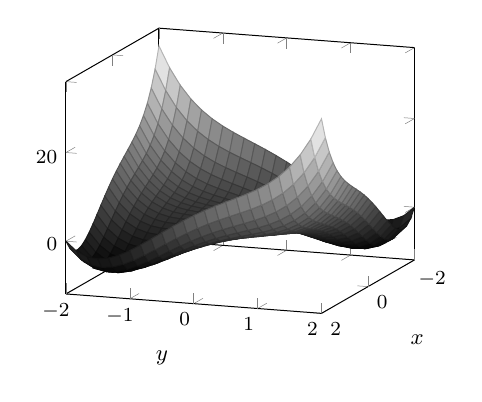
\begin{tikzpicture}[scale=.9]
        \begin{axis}[
          colormap/blackwhite,
          % title={$x \exp(-x^2-y^2)$},
          % rotate = 180,
          xlabel=$x$, ylabel=$y$, %
          % xlabel style = {rotate = -90}, %
          small, %
          view = {110}{15}, %
          ] %
          \addplot3[ %
          surf, %
          domain=-2:2, %
          domain y=-2:2, %
          ] %
          {x^4 + y^4 - 2*(x-y)^2}; %
        \end{axis}
      \end{tikzpicture}
      & 
      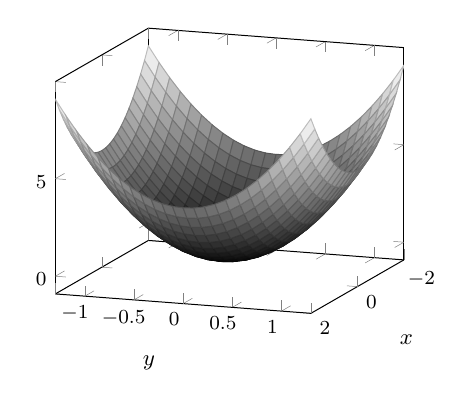
\begin{tikzpicture}[scale=.9]
        \begin{axis}[
          colormap/blackwhite,
          % title={$x \exp(-x^2-y^2)$},
          xlabel=$x$, ylabel=$y$, %
          small, %
          view = {110}{15}, %
          ] %
          \addplot3[ %
          surf, %
          domain=-2:2, %
          domain y=-1.3:1.3, %
          ] %
          {x^2 + 3 * y^2}; %
        \end{axis}
      \end{tikzpicture}
      &
      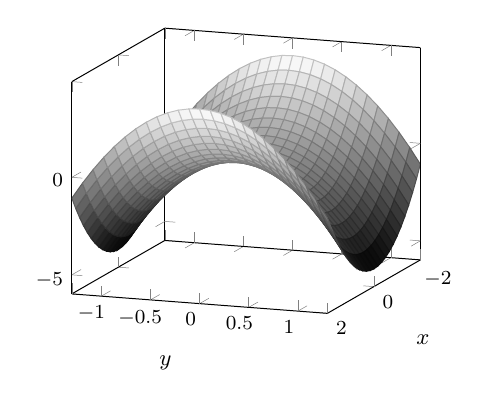
\begin{tikzpicture}[scale=.9]
        \begin{axis}[
          colormap/blackwhite,
          % title={$x \exp(-x^2-y^2)$},
          xlabel=$x$, ylabel=$y$, %
          small, %
          view = {110}{15}, %
          ] %
          \addplot3[ %
          surf, %
          domain=-2:2, %
          domain y=-1.3:1.3, %
          ] %
          {x^2-3*y^2}; %
        \end{axis}
      \end{tikzpicture}
      \nl
      Nappe $1$ & Nappe $2$ & Nappe $3$
    \end{array}
    \]
    
    
    \newpage
    
    
    \begin{proof}~%
      \begin{noliste}{$\sbullet$}
      \item D'après l'étude précédente, la fonction $f$ possède un
        minimum global réalisé en les deux points ($(\sqrt{2},
        -\sqrt{2})$, $(-\sqrt{2}, \sqrt{2})$).
      \item On peut écarter la deuxième nappe qui représente une
        fonction n'admettant un minimum global qu'en un point.
      \item On peut écarter la troisième nappe qui représente une
        fonction n'admettant pas de minimum global (elle admet par
        contre un point selle).
      \item Seule la première nappe représente une fonction admettant
        un minimum global réalisé en deux points. C'est donc la
        représentation de la fonction $f$ considéré.          
      \end{noliste}
      \conc{Le script précédent renvoie la première
        nappe.}%~\\[-1.2cm]
      \begin{remark}%~\\
        Il était difficile de lire les coordonnées des deux points
        atteignant le minimum sur l'énoncé original. Pour être certain
        d'avoir des points (même si la photocopie en noir et blanc
        rend le graphique peut lisible), il est conseillé de lister
        les propriétés que doit avoir la nappe représentant $f$.
      \end{remark}~\\[-1.4cm]
    \end{proof}
  \end{noliste}
\end{noliste}

\section*{Exercice 2}

\noindent
On note $E$ l'espace vectoriel des fonctions polynomiales de degré
inférieur ou égal à $2$ et on rappelle que la famille
$(e_{0},e_{1},e_{2})$ est une base de $E$, les fonctions $e_{0}$,
$e_{1}$ $e_{2}$ étant définies par :
\[
\forall t \in \R \quad e_{0}(t) = 1, \quad e_{1}(t) = t, \quad
e_{2}(t) = t^{2}
\]
On considère l'application $\varphi$ qui, à toute fonction $P$ de $E$,
associe la fonction, notée $\varphi(P)$, définie par :
\[
\forall x \in \R, \ \left(\varphi(P)\right)(x) = \dint{0}{1} P(x + t)
\ dt
\]
\begin{noliste}{1.}
 \setlength{\itemsep}{4mm}
\item
  \begin{noliste}{a)}
    \setlength{\itemsep}{2mm}
  \item Montrer que $\varphi$ est linéaire.

    \begin{proof}~\\
      Soit $(\lambda_1, \lambda_2) \in \R^2$ et soit $(P_1, P_2) \in
      E^2$. Soit $x \in \R$.
      \[
      \begin{array}{rcl@{\quad}>{\it}R{3.5cm}}
        \Big(\varphi(\lambda_1 \cdot P_1 + \lambda_2 \cdot P_2)\Big)(x) & = &
        \dint{0}{1} (\lambda_1 \cdot P_1 + \lambda_2 \cdot P_2)(x+t)
        \dt
        \\[.6cm]
        & = & \dint{0}{1} (\lambda_1 \cdot P_1(x+t) + \lambda_2 \cdot
        P_2(x+t)) \dt
        \\[.6cm]
        & = & \lambda_1 \ \dint{0}{1} P_1(x+t) \dt + \lambda_2 \
        \dint{0}{1} P_2(x+t) \dt & (par linéarité \\ de l'intégration)
        \nl
        \nl[-.2cm]
        & = & \lambda_1 \ (\varphi(P_1))(x) + \lambda_2 \
        (\varphi(P_2))(x)
        \\[.2cm]
        & = & \Big(\lambda_1 \cdot \varphi(P_1) + \lambda_2 \cdot
        \varphi(P_2)\Big) (x)
      \end{array}
      \]
      L'égalité précédente étant vérifiée pour tout réel $x$, on en
      déduit : 
      \[
      \varphi(\lambda_1 \cdot P_1 + \lambda_2 \cdot P_2) = \lambda_1
      \cdot \varphi(P_1) + \lambda_2 \cdot \varphi(P_2)
      \]
      \conc{L'application $\varphi$ est linéaire.}%~\\[-1cm]
      
      
      \newpage
      
      
      \begin{remark}%~
        \begin{noliste}{$\sbullet$}
        \item Cet exercice est de facture classique.\\
          La principale difficulté provient de la manipulation
          d'objets. Il faut donc bien prendre le temps de comprendre
          la définition de l'application $\varphi : E \to E$.
        \item Détaillons les objets considérés.
          \begin{noliste}{$-$}
          \item En accord avec le programme, les polynômes sont
            confondus avec leur application polynomiale
            associée. C'est ainsi que $e_0$, $e_1$ et $e_2$, éléments
            de $E$, sont définies en tant qu'application ($\forall t
            \in \R, \ e_{0}(t) = 1, \ e_{1}(t) = t, \ e_{2}(t) =
            t^{2}$).\\
            La variable $t$ utilisée ici est muette (on pourrait aussi
            bien définir ces applications par : $\forall u \in \R$,
            $e_0(u) = 1$, $e_{1}(u) = u$, $e_2(u) = u^2$) et n'a pas
            de lien avec la variable d'intégration (muette) nommée
            elle aussi $t$. Ces applications polynomiales sont parfois
            notées $P_0$, $P_1$ et $P_2$, la lettre $P$ étant
            traditionnellement utilisée pour désigner un polynôme (ce
            que fait l'énoncé).
          \item L'application $\varphi$ associe à toute application
            polynomiale $P$ une application polynomiale notée
            $\varphi(P)$. Une telle application est définie par sa
            valeur en tout point $x \in \R$ (nouvelle variable
            muette). C'est ce qui est fait dans l'énoncé qui fournit
            la valeur de $(\varphi(P))(x)$.
          \item Enfin, $\dint{0}{1} P(x+t) \dt$ est une quantité qui
            dépend de $x$ mais qui est indépendante de $t$, variable
            (muette) d'intégration.
          \end{noliste}
        \end{noliste}
      \end{remark}~\\[-1.2cm]
    \end{proof}
    
  \item Déterminer $\left(\varphi(e_{0})\right)(x)$,
    $\left(\varphi(e_{1})\right)(x)$ et
    $\left(\varphi(e_{2})\right)(x)$ en fonction de $x$, puis écrire
    $\varphi(e_{0})$, $\varphi(e_{1})$ et $\varphi(e_{2})$ comme
    combinaison linéaire de $e_{0}$, $e_{1}$ et $e_{2}$.

    \begin{proof}~\\
      Soit $x \in \R$.
      \begin{noliste}{$\sbullet$}
      \item Tout d'abord :
        \[
        (\varphi(e_0))(x) = \dint{0}{1} e_0(x+t) \dt = \dint{0}{1} 1
        \dt = 1 \ (1-0) = 1 = e_0(x)
        \]
        \conc{L'égalité précédente étant vérifiée pour tout réel $x$,
          on en déduit : $\varphi(e_0) = e_0$.}
      \item Ensuite :
        \[
        \begin{array}{rcl@{\quad}>{\it}R{3.5cm}}
          (\varphi(e_1))(x) & = & \dint{0}{1} e_1(x+t) \dt \ = \ \dint{0}{1}
          (x+t) \dt 
          \\[.6cm]
          & = & \dint{0}{1} x \dt + \dint{0}{1} t \dt & (par linéarité
          \\ de l'intégration)
          \nl
          \nl[-.2cm]
          & = & x \ (1-0) + \Prim{\dfrac{t^2}{2}}{0}{1}
          \\[.6cm]
          & = & x + \dfrac{1}{2} 
          \\[.2cm]
          & = & e_1(x) + \dfrac{1}{2} \ e_0(x) \ = \ \left(
            e_1 + \dfrac{1}{2} \ e_0 \right)(x)
        \end{array}
        \]
        \conc{L'égalité précédente étant vérifiée pour tout réel $x$,
          on en déduit : $\varphi(e_1) = e_1 + \dfrac{1}{2} \ e_0$.}


        \newpage


      \item Enfin :
        \[
        \begin{array}{rcl@{\quad}>{\it}R{3.5cm}}
          (\varphi(e_2))(x) & = & \dint{0}{1} e_2(x+t) \dt \ = \ \dint{0}{1}
          (x+t)^2 \dt 
          \\[.6cm]
          & = & \dint{0}{1} x^2 \dt + 2x \ \dint{0}{1} t \dt +
          \dint{0}{1} t^2 \dt & (par linéarité \\ de l'intégration)
          \nl
          \nl[-.2cm]
          & = & x^2 \ (1-0) + 2 \ x \Prim{\dfrac{t^2}{2}}{0}{1} +
          \Prim{\dfrac{t^3}{3}}{0}{1} 
          \\[.6cm]
          & = & x^2 + x + \dfrac{1}{3} 
          \\[.2cm]
          & = & e_2(x) + e_1(x) + \dfrac{1}{3} \ e_0(x) \ = \ \left(
            e_2 + e_1 + \dfrac{1}{3} \ e_0 \right)(x)
        \end{array}
        \]
        \conc{L'égalité précédente étant vérifiée pour tout réel $x$,
          on en déduit : $\varphi(e_2) = e_2 + e_1 + \dfrac{1}{3} \
          e_0$.}~\\[-1.2cm]
      \end{noliste}
    \end{proof}

  \item Déduire des questions précédentes que $\varphi$ est un
    endomorphisme de $E$.

    \begin{proof}~%
      \begin{noliste}{$\sbullet$}
      \item D'après la question \itbf{1.a)}, l'application $\varphi$
        est linéaire.

      \item Il reste à démontrer que cette application est à valeurs
        dans $E$.\\
        Soit $P \in E$. Comme $(e_0, e_1, e_2)$ est une base de $E$,
        il existe un unique triplet $(a_0, a_1, a_2) \in \R^3$ tel que
        :
        \[
        P = a_0 \ e_0 + a_1 \ e_1 + a_2 \ e_2
        \]
        Ainsi :
        \[
        \begin{array}{rcl@{\quad}>{\it}R{3.5cm}}
          \varphi(P) & = & \varphi(a_0 \ e_0 + a_1 \ e_1 + a_2 \ e_2)
          \\[.2cm]
          & = & a_0 \ \varphi(e_0) + a_1 \  \varphi(e_1) + a_2 \
          \varphi(e_2) & (par linéarité de $\varphi$)
          \nl
          \nl[-.2cm]
          & = & a_0 \ e_0 + a_1 \ \left( \dfrac{1}{2} \ e_0 + e_1
          \right) + a_2 \ \left( \dfrac{1}{3} \ e_0 + e_1 + e_2\right)
          & (d'après la \\ question précédente)
          \nl
          \nl[-.2cm]
          & = & \left( a_0 + \dfrac{1}{2} a_1 + \dfrac{1}{3} a_2
          \right) \ e_0 + \left( a_1 + a_2 \right) \ e_1 + a_2 \ e_2
        \end{array}
        \]
        Ainsi, $\varphi(P) \in \Vect{e_0, e_1, e_2} = E$.
      \end{noliste}
      \conc{On en déduit que $\varphi$ est un endomorphisme de $E$.}
      \begin{remark}%~\\
        On aurait aussi pu calculer directement $\varphi(P)$ :
        \[
        \begin{array}{rcl}
          (\varphi(P))(x) & = & \dint{0}{1} P(x+t) \dt = \dint{0}{1} \left(
            a_0 + a_1 \ (x+t) + a_2 \ (x+t)^2 \right) \dt
          \\[.6cm]
          & = & \ldots \ = \ \left( a_0 + \dfrac{1}{2} a_1 + \dfrac{1}{3} a_2
          \right) + \left( a_1 + a_2 \right) \ x + a_2 \ x^2
        \end{array}
        \]
        Mais ce n'était pas l'esprit du sujet et cela obligeait à
        refaire des calculs déjà effectués précédemment.
      \end{remark}~\\[-1cm]
    \end{proof}
  \end{noliste}
  
  
  \newpage
  
  
\item
  \begin{noliste}{a)}
    \setlength{\itemsep}{2mm}
  \item Écrire la matrice $A$ de $\varphi$ dans la base
    $(e_{0},e_{1},e_{2})$. On vérifiera que la première ligne de $A$
    est :
    \[
    \begin{smatrix}
      1 & \dfrac{1}{2} & \dfrac{1}{3}
    \end{smatrix}
    \]

    \begin{proof}~\\%
      D'après la question \itbf{1.b)} :
      \begin{noliste}{$\sbullet$}
      \item $\varphi(e_0) = 1 \cdot e_0 + 0 \cdot e_1 + 0 \cdot e_2$.\\
        Ainsi : $\Mat_{(e_0, e_1, e_2)}(\varphi(e_0)) =
        \begin{smatrix}
          1 \\
          0 \\
          0
        \end{smatrix}
        $.

      \item $\varphi(e_1) = \dfrac{1}{2} \cdot e_0 + 1 \cdot e_1 + 0
        \cdot e_2$.\\ 
        Ainsi : $\Mat_{(e_0, e_1, e_2)}(\varphi(e_1)) =
        \begin{smatrix}
          \frac{1}{2} \\
          1 \\
          0
        \end{smatrix}
        $.

      \item $\varphi(e_2) = \dfrac{1}{3} \cdot e_0 + 1 \cdot e_1 + 1
        \cdot e_2$.\\ 
        Ainsi : $\Mat_{(e_0, e_1, e_2)}(\varphi(e_2)) =
        \begin{smatrix}
          \frac{1}{3} \\
          1 \\
          1
        \end{smatrix}
        $.        
      \end{noliste}
      \conc{On en déduit : $A = \Mat_{(e_0, e_1, e_2)}(\varphi) =
        \begin{smatrix}
          1 & \frac{1}{2} & \frac{1}{3} \\
          0 & 1 & 1 \\
          0 & 0 & 1
        \end{smatrix}
        $.}~\\[-1cm]
    \end{proof}

  \item Justifier que $\varphi$ est un automorphisme de $E$.

    \begin{proof}~\\
      La matrice $A$ est inversible car elle est triangulaire
      supérieure et ses coefficients diagonaux sont tous non
      nuls. La matrice $A$ étant la représentation matricielle dans la
      base $(e_0, e_1, e_2)$ de $\varphi$, on en déduit que $\varphi$
      est bijective.%
      \conc{Ainsi, $\varphi$ est un automorphisme de $E$.}~\\[-1.2cm]
    \end{proof}

  \item L'endomorphisme $\varphi$ est-il diagonalisable ?

    \begin{proof}~%
      \begin{noliste}{$\sbullet$}
      \item La matrice $A$ est triangulaire supérieure. \\
        Ses valeurs propres sont donc ses coefficients diagonaux.%
        \conc{On en conclut : $\spc(\varphi) = \spc(A) = \{1\}$.}

      \item Montrons par l'absurde que $\varphi$ n'est pas diagonalisable.\\
        Supposons que $\varphi$ est diagonalisable, alors $A =
        \Mat_{(e_0, e_1, e_2)}(\varphi)$ l'est aussi.\\
        Il existe donc une matrice inversible $P \in \M{3}$ et une
        matrice diagonale $D \in \M{3}$ dont les coefficients
        diagonaux sont les valeurs propres de $A$ telles que $A =
        PDP^{-1}$.\\
        Or $1$ est la seule valeur propre de $A$. Ainsi $D = I$ et :
        \[
        A = PDP^{-1} = PIP^{-1} = PP^{-1} = I
        \]
        Absurde !%
%         Supposons par l'absurde que $\varphi$ est diagonalisable.\\
%         Il existe alors une base $\B'$ de $E$ dans laquelle la matrice
%         représentative de $\varphi$ est diagonale et dont les
%         coefficients diagonaux sont tous $1$ (seule valeur propre de
%         $\varphi$). Ainsi :
%         \[
%         \Mat_{\B'}(\varphi) =
%         \begin{smatrix}
%           1 & 0 & 0 \\
%           0 & 1 & 0 \\
%           0 & 0 & 1
%         \end{smatrix}
%         = I_3
%         \]
%         On en déduit, par la formule de changement de base (en notant
%         $\B = (e_0, e_1, e_2)$) :
%         \[
%         \begin{array}{rcl}
%           A \ = \ \Mat_{\B}(\varphi) & = & P_{\B, \B'} \times
%           \Mat_{\B'}(\varphi) 
%           \times (P_{\B, \B'})^{-1} 
%           \\[.2cm]
%           & = & P_{\B, \B'} \times I_3 \times (P_{\B, \B'})^{-1} \ = \ I_3
%         \end{array}       
%         \]
%         Impossible car $A \neq I_3$.
        \conc{L'endomorphisme $\varphi$ n'est pas diagonalisable.}


        \newpage


        \begin{remark}%~%
          \begin{noliste}{$\sbullet$}
          \item Il était possible de déterminer $E_1(\varphi)$
            l'espace propre associé à $1$.
          \item Détaillons la rédaction associée.\\
            Soit $P = a_0 \ e_0 + a_1 \ e_1 + a_2 \ e_2 \in E$ . On a
            alors $U = \Mat_{\B}(P) =
            \begin{smatrix}
              a_0 \\
              a_1 \\
              a_2
            \end{smatrix}
            $.
            \[
            \begin{array}{rcl}
              P \in E_1(\varphi) 
              & \Longleftrightarrow & (\varphi - \id_E)(P) = 0_E 
              \\[.2cm]
              & \Longleftrightarrow & (A - I_3) \ U = 0_{\M{31}}
              \\[.2cm]
              & \Longleftrightarrow & 
              \left\{
                \begin{array}{rcrcrcr}
                  & & \frac{1}{2} \ a_1 & + & \frac{1}{3} \ a_2 & = & 0
                  \\[.2cm]
                  & & & & a_2 & = & 0
                  \\[.2cm]
                  & & & & 0 & = & 0
                \end{array}
              \right.
              \\[1cm]
              & \Longleftrightarrow & 
              \left\{
                \begin{array}{l}
                  a_1 = a_2 = 0
                \end{array}
              \right.
              \\[.2cm]
              & & \text{\it (par remontées successives)}
            \end{array}
            \]
            On en déduit :
            \[
            \begin{array}{rcl}
              E_1(\varphi) & = & \{ P = a_0 \ e_0 + a_1 \ e_1 + a_2 \ e_2 \
              | \ (\varphi - \id_E)(P) = 0_E \}
              \\[.2cm]
              & = & \{ a_0 \ e_0 + a_1 \ e_1 + a_2 \ e_2 \
              | \ a_1 = a_2 = 0 \}
              \\[.2cm]
              & = & \{ a_0 \ e_0 \ | \ a_0 \in \R \}
              \\[.2cm]
              & = & \Vect{e_0}
            \end{array}
            \]
            La famille ${\cal F} = (e_0)$ est génératrice de $E_1(\varphi)$.\\
            De plus, elle est libre car constituée d'un vecteur non
            nul.\\
            C'est donc une base de $E_1(\varphi)$ et
            $\dim(E_1(\varphi)) = \Card({\cal F}) = 1$.\\[.2cm]
            Comme : $\dim(E_1(\varphi)) = 1 \neq 3 = \dim(E)$, alors
            $\varphi$ n'est pas diagonalisable.
          \end{noliste}
        \end{remark}~\\[-1.4cm]
      \end{noliste}
    \end{proof}
  \end{noliste}

\item Compléter les commandes \Scilab{} suivantes pour que soit
  affichée la matrice $A^{n}$ pour une valeur de $n$ entrée par
  l'utilisateur :
  \begin{scilab}
    & n = input(\ttq{}entrez une valeur pour n : \ttq{}) \nl %
    & A = [------] \nl %
    & disp(------)
  \end{scilab}

  \begin{proof}~%
    \begin{noliste}{$\sbullet$}
    \item On stocke la matrice $A$ dans la variable {\tt A}.\\
      \begin{scilabC}{1}
        & A = [1, 1/2, 1/3; 0, 1, 1; 0, 0, 1]
      \end{scilabC}~

    \item Puis on demande l'affichage de $A^n$.
      \begin{scilabC}{2}
        & disp(A\puis{}n)
      \end{scilabC}
    \end{noliste}
  \end{proof}


\newpage


\item
  \begin{noliste}{a)}
    \setlength{\itemsep}{2mm}
  \item Montrer par récurrence que, pour tout entier naturel $n$, il
    existe un réel $u_{n}$ tel que l'on ait :
    \[
    A^{n} = 
    \begin{smatrix}
      1 & \frac{n}{2} & u_{n}\\
      0 & 1 & n\\
      0 & 0 & 1
    \end{smatrix}
    \]
    Donner $u_{0}$ et établir que : $\forall n \in \N, \ u_{n + 1} =
    u_{n} + \dfrac{1}{6}\left(3n + 2\right)$.
    
    \begin{proof}~\\
      Démontrons par récurrence : $\forall n \in \N$, $\PP{n}$
      \\
      où \ $\PP{n}$ : il existe un réel $u_n$ tel que $A^n =
      \begin{smatrix}
        1 & \frac{n}{2} & u_{n}\\
        0 & 1 & n\\
        0 & 0 & 1
      \end{smatrix}$.
      \begin{noliste}{\fitem}
      \item {\bf Initialisation} :
        \begin{noliste}{$\sbullet$}
        \item Tout d'abord : $A^0 = I_3$.
        \item Par ailleurs : $\begin{smatrix}
            1 & \frac{0}{2} & u_{0}\\
            0 & 1 & 0\\
            0 & 0 & 1
          \end{smatrix} 
          = 
          \begin{smatrix}
            1 & 0 & u_{0}\\[.1cm]
            0 & 1 & 0\\
            0 & 0 & 1
          \end{smatrix}$
        \end{noliste}
        Notons alors $u_0 = 0$. On a bien démontré l'existence d'un
        réel $u_0$ tel que : $A^{0} =
        \begin{smatrix}
          1 & \frac{0}{2} & u_{0}\\
          0 & 1 & 0\\
          0 & 0 & 1
        \end{smatrix}$.\\
        D'où $\PP{0}$.

      \item {\bf Hérédité} : soit $n \in \N$.\\
        Supposons $\PP{n}$ et démontrons $\PP{n+1}$ (il existe
        $u_{n+1} \in \R$ tel que $ A^{n+1} = 
        \begin{smatrix}
          1 & \frac{n+1}{2} & u_{n+1}\\
          0 & 1 & n+1 \\
          0 & 0 & 1
        \end{smatrix}$).
        \begin{noliste}{$\sbullet$}
        \item Par hypothèse de récurrence, il existe $u_n \in \R$ tel
          que :
          \[
          A^n =
          \begin{smatrix}
            1 & \frac{n}{2} & u_{n} \\
            0 & 1 & n \\
            0 & 0 & 1
          \end{smatrix}          
          \]
          On en déduit :
          \[
          \begin{array}{rcl}
            A^{n+1} & = & A \ A^n 
            \\[.2cm]
            & = &            
            \begin{smatrix}
              1 & \frac{1}{2} & \frac{1}{3} \\
              0 & 1 & 1 \\
              0 & 0 & 1
            \end{smatrix}          
            \begin{smatrix}
              1 & \frac{n}{2} & u_{n} \\
              0 & 1 & n \\
              0 & 0 & 1
            \end{smatrix}          
            \\[.8cm]
            & = &
            \begin{smatrix}
              1 & \frac{n}{2} + \frac{1}{2} & u_n + \frac{n}{2} +
              \frac{1}{3} \\
              0 & 1 & n+1 \\
              0 & 0 & 1
            \end{smatrix}
          \end{array}          
          \]
          Notons alors $u_{n+1} = u_n + \frac{n}{2} + \frac{1}{3}$.\\
          On a bien démontré l'existence d'un réel $u_{n+1}$ tel que :
          $A^{n+1} =
          \begin{smatrix}
            1 & \frac{n+1}{2} & u_{n+1}\\
            0 & 1 & n+1\\
            0 & 0 & 1
          \end{smatrix}$.\\
          D'où $\PP{n+1}$.
        \end{noliste}        
      \end{noliste}
      \conc{Par principe de récurrence : $\forall n \in \N$,
        $\PP{n}$.}%
      \conc{En particulier : $u_0 = 0$ et pour tout $n \in \N$,
        $u_{n+1} = u_n + \dfrac{n}{2} + \dfrac{1}{3} = u_n +
        \dfrac{1}{6} \ (3n + 2)$.}~\\[-1cm]
    \end{proof}


    \newpage


  \item En déduire, par sommation, l'expression de $u_{n}$ pour tout
    entier $n$.

    \begin{proof}~%
      \begin{noliste}{$\sbullet$}
      \item D'après la question précédente, pour tout $k \in \N$ :
        \[
        u_{k+1} - u_k = \dfrac{1}{6} \ (3k + 2)
        \]
      \item On en déduit que pour tout $n \in \N^*$ : 
        \[
        \begin{array}{rcl}
          \Sum{k=0}{n-1} (u_{k+1} - u_k) & = & \Sum{k=0}{n-1}
          \dfrac{1}{6} \ (3k + 2) 
          \\[.6cm]
          & = & \dfrac{1}{6} \ \Sum{k=0}{n-1} (3k + 2) 
          \\[.6cm]
          & = & \dfrac{1}{6} \ \left(3 \ \Sum{k=0}{n-1} k +
            \Sum{k=0}{n-1} 2 \right) 
          \\[.6cm]
          & = & \dfrac{1}{6} \ \big(3 \ \dfrac{n(n-1)}{2} + 2 n \big) 
          \\[.6cm]
          & = & \dfrac{1}{12} \ \big(3 \ n(n-1) + 4 n \big) 
          \\[.6cm]
          & = & \dfrac{1}{12} \ \Big( n \big(3 \ (n-1) + 4 \big) \Big) 
          \\[.6cm]
          & = & \dfrac{n \ (3n+1)}{12}
        \end{array}
        \]
      \item Par ailleurs :  
        \[
        \Sum{k=0}{n-1} (u_{k+1} - u_k) = u_n - u_0 = u_n
        \]        
      \item On en déduit : 
        \[ 
        \forall n \in \N^*, \ u_n = \dfrac{n \ (3n+1)}{12}
        \] 
        Cette relation est aussi vraie pour $n = 0$. En effet :
        \begin{noliste}{$\stimes$}
        \item d'une part : $u_0 = 0$,
        \item d'autre part : $\dfrac{0 \ (3 \times 0+1)}{12} = 0$.
        \end{noliste} 
        % Cette relation est aussi vraie pour $n = 0$ puisque : $u_0 =
        % 0$ et $\dfrac{0 \ (3 \times 0+1)}{12} = 0$.
      \end{noliste}
      \conc{Ainsi : $\forall n \in \N$, $u_n = \dfrac{n \
          (3n+1)}{12}$.}~\\[-1cm]
    \end{proof}


    \newpage


  \item Écrire $A^{n}$ sous forme de tableau matriciel.

    \begin{proof}~%
      \conc{D'après les questions précédentes : $A^n =
        \begin{smatrix}
          1 & \dfrac{n}{2} & \dfrac{n \ (3n+1)}{12} \\[.2cm]
          0 & 1 & n \\
          0 & 0 & 1
        \end{smatrix}$.}
      \begin{remark}%~
        Cette question peut dérouter puisque le terme \og tableau
        matriciel \fg{} n'est pas habituel. C'est simplement
        l'occasion, pour les candidats ayant réussi la question
        précédente, de prendre des points supplémentaires.
      \end{remark}~\\[-1.2cm]
    \end{proof}
 \end{noliste}
\end{noliste} 


\newpage


\section*{Exercice 3}

\noindent
Soit $V$ une variable aléatoire suivant la loi exponentielle de
paramètre $1$, dont la fonction de répartition est la fonction $F_{V}$
définie par : $F_{V}(x) = \left\{
  \begin{array}{cl}
    0 & \hbox{ si } x \leq 0\\
    1-\ee^{-x} & \hbox{ si } x>0 
  \end{array}
\right.$.\\
On pose $W = -\ln(V)$ et on admet que $W$ est aussi une variable
aléatoire dont le fonction de répartition est notée $F_{W}$. On dit
que $W$ suit une loi de Gumbel.
\begin{noliste}{1.}
  \setlength{\itemsep}{4mm}
\item
  \begin{noliste}{a)}
    \setlength{\itemsep}{2mm}
  \item Montrer que : $\forall x \in \R, \ F_{W}(x) =
    \ee^{-\ee^{-x}}$.
    
    \begin{proof}~
      \begin{noliste}{$\sbullet$}
      \item Notons $h : x \mapsto -\ln(x)$, de sorte que $W = h(V)$.\\
        Comme $V \suit \Exp{1}$, alors $V(\Omega) = \ ]0,+\infty[$. On
        en déduit :
        \[
        \begin{array}{rcl@{\qquad}>{\it}R{6cm}}
          W(\Omega) & = & \multicolumn{2}{l}{h(V) \hspace{.08cm} (\Omega)
            % \\[.2cm]
            \ = \ h\big( V(\Omega) \big) }
          \\[.2cm]
          & = & h\big( ]0, +\infty[ \big)
          \\[.2cm]
          & = & ]\dlim{x \tend +\infty} h(x), \dlim{x \tend 0} h(x)[
          & (car $h$ est continue et strictement décroissante
          sur $]0, +\infty[$)
          \nl
          \nl[-.2cm]
          & = & ]-\infty, +\infty[ & (car $\dlim{x \tend +\infty}
          -\ln(x) = -\infty$ \\ et $\dlim{x \tend 0} - \ln(x) = +\infty$)
        \end{array}
        \]
% On
%         a les équivalences suivantes :
% 	\[
% 	 \begin{array}{rcl@{\qquad}>{\it}R{4cm}}
%            x \in V(\Omega) & \Leftrightarrow & x \in \ ]0,+\infty[
%            \\[.2cm]
%            & \Leftrightarrow & 0<x<+\infty
%            \\
%            & \Leftrightarrow & -\infty < \ln(x) < +\infty & (car la 
%            fonction $\ln$ est strictement croissante sur $\R_+^*$)
%            \nl[-.4cm]
%            \nl
%            & \Leftrightarrow & +\infty > -\ln(x) > -\infty
%            \\[.2cm]
%            & \Leftrightarrow & +\infty > f(x) > -\infty
%            \\[.2cm]
%            & \Leftrightarrow & f(x) \in \R
% 	 \end{array}
% 	\]
% 	%Ainsi :
% 	\[
% 	 \begin{array}{R{2cm}rcl@{\qquad}>{\it}R{5cm}}
%            Ainsi : & W(\Omega) & = & f(V)(\Omega)
%            \\%[.2cm]
%            & & = & \{f(x) \ | \ x \in V(\Omega)\}
%            % \\
%            \ = \ \R & (d'après les équivalences précédentes)
% 	 \end{array}
% 	\]
	\conc{Ainsi, $W(\Omega)=\R$.}
      \item Déterminons la fonction de répartition de $W$. Soit $x
        \in \R$.
	\[
        \begin{array}{rcl@{\qquad}>{\it}R{5.5cm}}
          F_W(x) & = & \multicolumn{2}{l}{\Prob(\Ev{W\leq x})
            \ = \ \Prob(\Ev{-\ln(V)\leq x})}
          \\[.2cm]
          & = & \Prob(\Ev{\ln(V) \geq -x})
          \\%[.2cm]
          & = & \Prob(\Ev{V\geq \ee^{-x}}) & (car la fonction $\exp$
          est strictement croissante sur $\R$)
          \nl
          \nl[-.4cm]
          & = & 1-\Prob(\Ev{V <\ee^{-x}})
          \\[.2cm]
          & = & 1-F_V(\ee^{-x}) & (car $V$ est une \var à densité)
          \nl[-.4cm]
          \nl
          & = & \bcancel{1}-\left(\bcancel{1}-\ee^{-\ee^{-x}}\right) & 
          (car $\ee^{-x} > 0$)
          \nl
          \nl[-.2cm]
          & = & \ee^{-\ee^{-x}} \\[-.4cm]
        \end{array}
	\]
      \end{noliste}
      \conc{$\forall x \in\R$, $F_W(x)=\ee^{-\ee^{-x}}$}~\\[-1.4cm]
      \begin{remark}%~
        \begin{noliste}{$\sbullet$}
        \item Commencer par déterminer l'ensemble image $V(\Omega)$
          est un bon réflexe : cela peut guider l'étude de la fonction
          de répartition $F_V$. Plus précisément, cela fournit la
          disjonction de cas à effectuer. Typiquement, si l'on
          démontre que $V(\Omega)$ est de la forme $[a, b]$ (où $a$ et
          $b$ sont deux réels tels que $a < b$), on peut rédiger comme
          suit :
          \begin{noliste}{$\stimes$}
          \item \dashuline{si $x < a$} alors $\Ev{V \leq x} =
            \emptyset$.\\
            Ainsi, $F_V(x) = \Prob(\Ev{V \leq x}) = \Prob(\emptyset) =
            0$.
          \item \dashuline{si $x \in [a, b]$} alors [\ldots {\tt démo
              à produire} \ldots]
          \item \dashuline{si $x > b$} alors $\Ev{X \leq x} =
            \Omega$.\\
            Ainsi, $F_V(x) = \Prob(\Ev{V \leq x}) = \Prob(\Omega) =
            1$.            
          \end{noliste}
        \item Les ensembles images $V(\Omega)$ de types différents
          (essentiellement $]-\infty, b]$ et $[a, +\infty[$) amènent
          des disjonctions de cas analogues.
%         \item On s'est permis, lors de l'écriture des premières
%           équivalences, d'écrire des inégalités comme $0 < x <
%           +\infty$ en lieu et place de $x \in \ ]0, +\infty[$. L'idée
%           derrière cette présentation est d'automatiser la
%           détermination des ensembles images.
        \end{noliste}
      \end{remark}~\\[-1.2cm]
    \end{proof}
    

    \newpage


  \item En déduire que $W$ est une variable à densité.
  
  \begin{proof}~\\
      La fonction de répartition $F_W$ est :
      \begin{noliste}{$\stimes$}
      \item continue sur $\R$ (car elle est la composée de fonctions
        continues sur $\R$).
      \item de classe $\Cont{1}$ sur $\R$ (car elle est la composée de
        fonctions de classe $\Cont{1}$ sur $\R$).
      \end{noliste}
      % ($x\mapsto \ee^{-x}$).
      \conc{Ainsi, $W$ est une variable à densité.}~\\[-1.2cm]
      % \begin{remark}%~\\
      %   La fonction $F_W : x \mapsto \Prob(\Ev{W \leq x})$ est, par
      %   définition, une fonction de répartition. Elle vérifie donc les
      %   propriétés des fonctions de répartition. Notamment 
      % \end{remark}
    \end{proof}
  \end{noliste}
\end{noliste}

\begin{noliste}{$\sbullet$}
\item On désigne par $n$ un entier naturel non nul et par $X_{1},
  \ldots, X_{n}$ des variables aléatoires définies sur le même espace
  probabilisé, indépendantes et suivant la même loi que $V$, c'est à
  dire la loi $\Exp{1}$.

\item On considère la variable aléatoire $Y_{n}$ définie par $Y_{n} =
  \max(X_{1},X_{2}, \ldots,X_{n})$, c'est à dire que pour tout
  $\omega$ de $\Omega$, on a : $Y_{n}(\omega) =
  \max(X_{1}(\omega),X_{2}(\omega), \ldots, X_n(\omega))$.\\
  On admet que $Y_{n}$ est une variable aléatoire à densité.
\end{noliste}

\begin{noliste}{1.}
  \setlength{\itemsep}{4mm} %
  \setcounter{enumi}{1}
\item
  \begin{noliste}{a)}
    \setlength{\itemsep}{2mm}
  \item Montrer que la fonction de répartition $F_{Y_{n}}$ de $Y_{n}$
    est définie par :
    \[
    F_{Y_{n}}(x) = \left\{
      \begin{array}{cl}
        0 & \hbox{ si } x<0\\
        (1-\ee^{-x})^{n} & \hbox{ si } x \geq 0
      \end{array}
    \right.
    \]
    
    \begin{proof}~
      \begin{noliste}{$\sbullet$}
      \item Déterminons tout d'abord $Y_n(\Omega)$.\\
	Pour tout $i\in\llb 1,n\rrb$, la \var $X_i$ suit la loi
        $\Exp{1}$, et donc $X_i(\Omega)=[0,+\infty[$.\\
        On rappelle que $Y_n= \max(X_1,\hdots, X_n)$. 
        % Les \var $X_i$ étant {\bf indépendantes}, $Y_n$ admet pour
        % ensemble image $Y_n(\Omega) = [0,+\infty[$.%
        \conc{Ainsi, $Y_n(\Omega) \ \subset \ [0,+\infty[$.}
	
      \item Soit $x \in \R$. Deux cas se présentent.
	\begin{noliste}{$-$}
        \item \dashuline{Si $x < 0$} : alors $\Ev{Y_n\leq x} =
          \varnothing$.
          % car $Y_n(\Omega)=[0,+\infty[$.
          Ainsi :
	  \[
          F_{Y_n}(x) \ = \ \Prob(\Ev{Y_n\leq x}) \ = \
          \Prob(\varnothing) \ = \ 0
	  \]

	  \item \dashuline{Si $x \geq 0$} :
	  \[
	    \begin{array}{rcl@{\qquad}>{\it}R{4cm}}
              F_{Y_n}(x) & = & \Prob(\Ev{Y_n\leq x})
              \\[.2cm]
              & = & \Prob(\Ev{\max(X_1,\hdots,X_n) \leq x})
              \\[.2cm]
              & = & \Prob(\Ev{X_1 \leq x} \ \cap \ \cdots \ \cap \Ev{X_n 
                \leq x})
              \\[.2cm]
              & = & \Prob(\Ev{X_1 \leq x}) \times \cdots \times 
              \Prob(\Ev{X_n \leq x}) & (car les \var $X_i$ \\ sont 
              indépendantes)
              \nl[-.2cm]
              \nl
              & = & \left( \Prob(\Ev{X_1\leq x}\right)^n & (car les \var
              $X_i$ \\ ont même loi)
              \nl[-.2cm]
              \nl
              & = & \left( 1-\ee^{-x}\right)^n & (car $X_1 \suit 
              \Exp{1}$)
	    \end{array}
	  \]
	  \conc{$\forall x \in\R$, $F_{Y_{n}}(x) = \left\{
	  \begin{array}{cl}
	    0 & \hbox{ si } x<0\\
	    (1-\ee^{-x})^{n} & \hbox{ si } x \geq 0
	  \end{array}
	  \right.$}%
	\end{noliste}
      \end{noliste}
      \begin{remark}%~\\
        \begin{noliste}{$\sbullet$}
        \item Cette question permet d'illustrer l'intérêt de la
          détermination de $Y_n(\Omega)$ : cela nous fournit la
          disjonction de cas servant à déterminer la fonction de
          répartition $F_{Y_n}$.
        \item On notera au passage que démontrer l'inclusion
          $Y_n(\Omega) \subset [0, +\infty[$ est suffisant pour mettre
          en place cette disjonction de cas.
        \end{noliste}
      \end{remark}~\\[-1.4cm]
    \end{proof}

    
    \newpage

    
  \item En déduire une densité $f_{Y_{n}}$ de $Y_{n}$.
    
    \begin{proof}~
      \begin{noliste}{$\sbullet$}
      \item $Y_n$ est une variable à densité car :
        \begin{noliste}{$\stimes$}
	\item $F_{Y_n}$ est continue sur $\R$.
	\item $F_{Y_n}$ est de classe $\Cont{1}$ sur $\R$, sauf
          éventuellement en $0$.\\[.2cm]
          En effet, sur $]-\infty,0[$, $F_{Y_n}$ est de classe
          $\Cont{1}$ car elle est constante sur cet intervalle.\\
          Sur $]0,+\infty[$, $F_{Y_n}$ est de classe $\Cont{1}$ car
          elle est la composée de fonctions de classe $\Cont{1}$ sur
          $\R$.
        \end{noliste}
      
      \item Pour déterminer une densité de $Y_n$, on dérive $F_{Y_n}$
        sur les {\bf intervalles ouverts}.\\
        Soit $x \in \R$. 
        \begin{noliste}{$-$}
        \item \dashuline{Si $x\in \ ]-\infty,0[$} :
          \[
          f_{Y_n}(x) = F_{Y_n}'(x) = 0
          \]
          
        \item \dashuline{Si $x\in \ ]0,+\infty[$} : 
          \[
          f_{Y_n}(x) = F_{Y_n}'(x) = n\ee^{-x}(1-\ee^{-x})^{n-1}
          \]
          
        \item \dashuline{Si $x = 0$} : on pose $f_{Y_n}(0)=0$.
        \end{noliste}
        \conc{$\forall x\in\R$, $f_{Y_n}(x)= \left\{
            \begin{array}{cl}
              0 & \hbox{ si } x\leq 0\\
              n\ee^{-x}(1-\ee^{-x})^{n-1} & \hbox{ si } x > 0
            \end{array}
          \right.$}%~\\[-1.6cm]
      \end{noliste}
      \begin{remark}%~%
        Il faut bien comprendre qu'on peut prendre n'importe quelle
        valeur positive pour $f_n$ en $0$. On peut ainsi construire
        une infinité de densités de $Y_n$. \\
        C'est pourquoi on parle d'{\bf une} densité.
      \end{remark}~\\[-1.2cm]
    \end{proof}
  \end{noliste}
  
\item
  \begin{noliste}{a)}
    \setlength{\itemsep}{2mm}
  \item Donner un équivalent de $1-F_{Y_{n}}(t)$ lorsque $t$ est au
    voisinage de $ + \infty$, puis montrer que l'intégrale $
    \dint{0}{+ \infty} \left(1-F_{Y_{n}}(t) \right) \ dt$ est
    convergente.
    
    \begin{proof}~\\
      On commence par déterminer un équivalent de $1-F_{Y_n}(t)$ quand
      $t\to +\infty$.
      \begin{noliste}{$\sbullet$}
      \item Soit $t\geq 0$.
        \[
        \begin{array}{rcl}
          F_{Y_n}(t) & = & \big(1-\ee^{-t} \big)^n
        \end{array}
        \]%~\\[-.5cm]
      \item On reconnaît une expression de la forme $(1+x)^\alpha$
        dont on connaît un développement limité en $0$. Plus
        précisément, il existe une fonction $\eps$ définie dans un
        voisinage de $0$ et qui vérifie $\dlim{x \tend 0} \eps(x) =
        0$, telle que, au voisinage de $0$ :
        \[
        (1 + x)^{n} \ = \ 1 + n \ x + x \ \eps(x)
        \]

      \item Comme $-\ee^{-t} \tendd{t}{+\infty} 0$, on peut appliquer
        l'égalité précédente à $x = -\ee^{-t}$ pour $t$ dans un
        voisinage de $+\infty$. On obtient :
        \[
        \begin{array}{C{1cm}rcl@{\qquad}>{\it}R{4.3cm}}
          & \left(1 -\ee^{-t} \right)^{n} & = & 1 - n \
          \ee^{-t} - \ee^{-t}\ \eps\left( -\ee^{-t} \right) 
          \\[.6cm]
          ainsi & 1 - \left(1 -\ee^{-t} \right)^{n} & = &
          n \ \ee^{-t} + \ee^{-t} \ \eps\left( -\ee^{-t} \right) 
          % \\[.6cm]
          % puis & \dfrac{1}{j^\alpha} \ \left(1 - \left(1 +
          %     \dfrac{1}{j} \right)^{n} \right) & = & 
          % \dfrac{1}{j^\alpha} \ \left(\alpha \ \dfrac{1}{j} -
          %   \dfrac{1}{j} \ \eps\left( -\ee^{-t} \right) \right) 
          % \\[.6cm]
          % enfin & j^{\alpha + 1} \ \Prob(\Ev{X = j}) & = & \alpha 
          % - \eps\left( -\ee^{-t} \right) 
          % & (par multiplication de part et d'autre par $j^{\alpha+1}$)
        \end{array}
        \]
      \item On constate alors : $\ee^{-t} \ \eps\left(
          -\ee^{-t} \right) = \oo{t}{+\infty} (\ee^{-t})$. En effet :
        \[
        \dfrac{\ee^{-t} \ \eps\left( -\ee^{-t} \right)}{\ee^{-t}} \ =
        \ \eps\left( -\ee^{-t} \right) \tendd{t}{+\infty} 0
        \]
        par théorème de composition des limites.

        % On reconnaît une expression de la forme $(1+x)^\alpha$ dont on 
%         connaît un développement limité (DL) à l'ordre $1$ en $0$ :
%         \[
%         (1+x)^\alpha = 1+\alpha x +\oox{0}(x)
%         \]
%         On applique ici ce DL à $\alpha=n$ et $x=-\ee^{-t}$, ce qui est 
%         autorisé car $\dlim{t\to+\infty} -\ee^{-t}=0$.\\ 
%         On obtient alors :
%         \[
%         \begin{array}{C{2.3cm}l}
%           & \big(1-\ee^{-t} \big)^n  = 1 -n\ee^{-t} + \oo{t}{+\infty}(\ee^{-t}) 
%           \\[.4cm]
%           d'où & 1-\big(1-\ee^{-t} \big)^n = n\ee^{-t} + \oo{t}{+\infty}(\ee^{-t}) 
%           \\[.4cm]
%           autrement dit & 1-F_{Y_n}(t) = n\ee^{-t} + \oo{t}{+\infty}(\ee^{-t})
%         \end{array}
%         \]
        % On obtient enfin :\\
        % \[
        % \dfrac{1-F_{Y_n}(t)}{n\ee^{-t}} = 1 + \oo{t}{+\infty} (1) 
        % \tendd{t}{+\infty} 1
        % \]~\\[-.5cm]


        \newpage


      \item On en conclut : $1-F_{Y_n}(t) = n \ \ee^{-t} +
        \oo{t}{+\infty}(\ee^{-t})$. %
        \conc{Et ainsi : $1-F_{Y_n}(t) \eq{t}{+\infty} n\ee^{-t}$.}
      \end{noliste}

      \noindent Démontrons alors que l'intégrale $\dint{0}{+ \infty}
      \left(1-F_{Y_{n}}(t) \right) \ dt$ est convergente.
      \begin{noliste}{$\sbullet$}       
      \item La fonction $t\mapsto 1-F_{Y_n}(t)$ est continue sur
        $[0,+\infty[$.
      \item D'autre part :
        \[
        1-F_{Y_n}(t) \eq{t}{+\infty} n\ \ee^{-t} \ (\geq 0)
        \]
      \item Or, l'intégrale $\dint{0}{+\infty} \ee^{-t} \dt$ est
        convergente (de la forme $\dint{0}{+\infty} \ee^{- \alpha t}
        \dt$ avec $\alpha > 0$).\\
        {\it (on ne change pas la nature d'une intégrale impropre en
          multipliant son intégrande par un réel non nul : ceci nous
          permet de ne pas prendre en compte le réel $n \neq 0$)}
      \end{noliste}
      Ainsi, par critère d'équivalence des intégrales impropres de
      fonctions continues positives, l'intégrale $\dint{0}{+\infty}
      (1-F_{Y_n}(t))\dt$ converge.%
      \conc{L'intégrale $\dint{0}{+\infty} (1-F_{Y_n}(t))\dt$ est
        convergente.}~\\[-.8cm]
      \begin{remark}%~%        
        \begin{noliste}{$\sbullet$}
        \item Les intégrales de type $\dint{0}{+\infty} \ee^{- \alpha
            t} \dt$ sont considérées dans le programme comme des
          intégrales de référence au même titre que les intégrales de
          Riemann ce qui explique la rédaction ci-dessus.
        \item On aurait pu justifier autrement la convergence de cette
          intégrale.
          \begin{noliste}{1)}
          \item \dashuline{Soit par calcul}.\\
            Soit $A\geq 0$.
            \[
            \dint{0}{A} n\ee^{-t}\dt = n\Prim{-\ee^{-t}}{0}{A}=
            n(1-\ee^{-A}) \tendd{A}{+\infty} n
            \]
            Donc $\dint{0}{+\infty} n\ee^{-t} \dt$ converge.

          \item \dashuline{Soit par un argument provenant du chapitre
              des \var à densité}.\\
            L'intégrale $\dint{0}{+\infty} \ee^{- t} \dt$ converge et
            vaut $1$ en tant qu'intégrale d'une densité d'une \var $X$
            suivant la loi exponentielle de paramètre $1$.
          \end{noliste}
        \end{noliste}
      \end{remark}~\\[-1.4cm]
    \end{proof}
      
  \item Établir l'égalité suivante :
    \[
    \forall x \in \R^+, \ \dint{0}{x} (1-F_{Y_{n}}(t)) \ dt =
    x\left(1-F_{Y_{n}}(x)\right) + \dint{0}{x} t f_{Y_{n}}(t) \ dt
    \]
    
    \begin{proof}~\\
      Soit $x\in\R_+$.
      % La fonction $F_{Y_n}$ est dérivable sur $\R_+$ de dérivée
      % $f_{Y_n}$.\\
      On procède par intégration par parties (IPP).
        \[
        \renewcommand{\arraystretch}{2}
        \begin{array}{|rcl@{\qquad}rcl}
          u(t) & = & 1-F_{Y_n}(t) & u'(t) & = & -f_{Y_n}(t) \\
          v'(t) & = & 1 & v(t) & = & t
        \end{array}
        \]
      Cette IPP est valide car les fonctions $u$ et $v$ sont 
      $\Cont{1}$ sur $[0, x]$. 


      \newpage

      
      \noindent
      On obtient alors :
      \[
       \begin{array}{rcl}
        \dint{0}{x} 1 \times (1-F_{Y_n}(t))\dt & = & \Prim{ 
	t \ (1-F_{Y_n}(t))}{0}{x} - \dint{0}{x} (-f_{Y_n}(t)) \times 
	t\dt
        \\[.4cm]
        & = & x \ (1-F_{Y_n}(x)) - \bcancel{0 \ (1-F_{Y_n}(0))}
         + \dint{0}{x} tf_{Y_n}(t) \dt
        \\[.4cm]
        & = & x \ (1-F_{Y_n}(x)) + \dint{0}{x} tf_{Y_n}(t) \dt
       \end{array}
      \]
      \conc{$\forall x \in\R_+$, $\dint{0}{x} (1-F_{Y_n}(t))\dt = 
      x(1-F_{Y_n}(x)) + \dint{0}{x} tf_{Y_n}(t)\dt$}~\\[-1cm]
    \end{proof}
    
  \item Montrer que : $\dlim{ x \to + \infty} x\left(1-F_{Y_{n}}(x)
    \right) = 0$.
    
    \begin{proof}~%
      \begin{noliste}{$\sbullet$}
      \item D'après la question \itbf{3.a)}, $1-F_{Y_n}(x)
        \eq{x}{+\infty} n\ee^{-x}$. On obtient alors :
        \[
        x(1-F_{Y_n}(x)) \eqx{+\infty} nx\ee^{-x}
        \]

      \item Or : $nx\ee^{-x} \tendx{+\infty} 0$.\\
        En effet, $x\ee^{-x} = \dfrac{x}{\ee^x} \tendx{+\infty} 0$ par
        croissances comparées. Ainsi : $nx\ee^{-x} \tendx{+\infty} 0$.
      \end{noliste}
      \conc{$\dlim{x\to+\infty} x(1-F_{Y_n}(x))=0$}~\\[-1.2cm]
    \end{proof}
    
  \item En déduire que $Y_{n}$ possède une espérance et prouver
    l'égalité :
    \[
    \E(Y_{n}) = \dint{0}{+ \infty} \left(1-F_{Y_{n}}(t)\right) \ dt
    \]~\\[-1.2cm]
    
    \begin{proof}~
      \begin{noliste}{$\sbullet$}
      \item La \var $Y_n$ admet une espérance si et seulement si
        l'intégrale impropre $\dint{-\infty}{+\infty} tf_{Y_n}(t)\dt$
        est absolument convergente, ce qui équivaut à démontrer la
        convergence pour les calculs de moment du type
        $\dint{-\infty}{+\infty} t^m f_{Y_n}(t)\dt$.\\
        Or : $\dint{-\infty}{+\infty} tf_{Y_n}(t)\dt =
        \dint{0}{+\infty} tf_{Y_n}(t)\dt$ car $f_{Y_n}$ est nulle en
        dehors de $[0, +\infty[$.
      \item Or, d'après la question \itbf{3.b)}, pour tout $x\geq 0$ :
      \[
      \dint{0}{x} tf_{Y_n}(t)\dt = \dint{0}{x}(1-F_{Y_n}(t)) \dt -
      x(1-F_{Y_n}(x)) %\qquad (*)
      \]
      La partie droite de l'égalité admet une limite finie quand $x
      \tend +\infty$ car :
      \begin{noliste}{$\stimes$}
      \item l'intégrale $\dint{0}{+\infty} (1-F_{Y_n}(t))\dt$ 
	converge, d'après la question \itbf{3.a)}
      \item $\dlim{x\to+\infty} x(1-F_{Y_n}(x))=0$, d'après la 
	question \itbf{3.b)}
      \end{noliste}
      On en déduit que l'intégrale $\dint{0}{+\infty} tf_{Y_n}(t)\dt$ est
      convergente. De plus :
      \[
      \dint{0}{+\infty} tf_{Y_n}(t)\dt =
      \dint{0}{+\infty}(1-F_{Y_n}(t)) \dt - 0
      \]
      \end{noliste}
%       \item Donc, en prenant la limite quand $x$ tend vers $+\infty$ 
%       dans l'équation $(*)$, on obtient que :
%       \begin{noliste}{$\stimes$}
% 	\item l'intégrale $\dint{0}{+\infty} tf_{Y_n}(t)\dt$ converge, 
% 	\ie $Y_n$ possède une espérance
% 	\item $\E(Y_n)$ vérifie l'égalité :
% 	\[
% 	 \E(Y_n) = 0 + \dint{0}{+\infty} (1-F_{Y_n}(t))\dt
% 	\]
%       \end{noliste}
      \conc{En conclusion, la \var $Y_n$ admet une espérance et
        $\E(Y_n) = \dint{0}{+\infty} (1-F_{Y_n}(t))\dt$.}~\\[-1cm]
    \end{proof}
  \end{noliste}


\newpage

  
\item
  \begin{noliste}{a)}
    \setlength{\itemsep}{2mm}
  \item Montrer, grâce au changement de variable $u = 1-\ee^{-t}$, que
    l'on a :
    \[
    \forall x \in \R^+, \ \dint{0}{x} \left(1-F_{Y_{n}}(t)\right) \ dt
    = \dint{0}{1 - \ee^{-x}} \dfrac{1-u^{n}}{1-u} \ du
    \]
    
    \begin{proof}~\\
      Soit $x\in\R_+$.
      \[
       \dint{0}{x} (1-F_{Y_n}(t))\dt = \dint{0}{x} 
       \left(1-\big(1-\ee^{-t} \big)^n\right) \dt
      \]
      On effectue le changement de variable $\Boxed{u = 1-\ee^{-t}}$. 
      % , où $\psi : t \mapsto 1-\ee^{-t}$ est de classe $\Cont{1}$
      % sur $[0,x]$.
      \[
      \left|
        \begin{array}{P{10cm}}
          $u = 1-\ee^{-t}$ (et donc $\ee^{-t} = 1-u$ puis $t = - \ln(1-u)$) \nl
          $\hookrightarrow$ $du = \ee^{-t}\dt$ \quad et \quad $dt
          = \dfrac{1}{\ee^{-t}}\ du = \dfrac{1}{1-u} \ du$ \nl
          \vspace{-.4cm}
          \begin{noliste}{$\sbullet$}
          \item $t = 0 \ \Rightarrow \ u = 0$
          \item $t = x \ \Rightarrow \ u = 1-\ee^{-x}$ %
            \vspace{-.4cm}
          \end{noliste}
        \end{array}
      \right.
      \]
      Ce changement de variable est valide car la fonction $\varphi :
      u \mapsto -\ln(1 - u)$ est $\Cont{1}$ sur $[0,1-\ee^{-x}]$.\\
      On remarque de plus que $u\in [0,1-\ee^{-x}]$, en particulier
      $u\neq 1$ (car $1-\ee^{-x}<1$ pour tout $x\geq 0$) ce qui permet
      de justifier la validité de l'écriture $\dfrac{1}{1-u}$.\\
      On obtient finalement :
      \[
      \dint{0}{x} \left(1-\big(1-\ee^{-t} \big)^n\right) \dt \ = \
      \dint{0}{1-\ee^{-x}} \left(1-u^n\right) \dfrac{1}{1-u} \ du \ =
      \ \dint{0}{1 - \ee^{-x}} \dfrac{1-u^{n}}{1-u} \ du
      \]
      \conc{$\forall x \in\R_+$, $\dint{0}{x} 
      \left(1-F_{Y_{n}}(t)\right) \ dt
      = \dint{0}{1 - \ee^{-x}} \dfrac{1-u^{n}}{1-u} \ du$}%~\\[-1cm]
    \end{proof}
    
  \item En déduire que : $ \dint{0}{x} \left(1-F_{Y_{n}}(t)\right) \
    dt = \Sum{k = 1}{n} \dfrac{(1-\ee^{-x})^{k}}{k}$ puis donner
    $\E(Y_{n})$ sous forme de somme.
    
    \begin{proof}~
      \begin{noliste}{$\sbullet$}
      \item On remarque tout d'abord : $u\in [0,1-\ee^{-x}]$. On a
        donc, en particulier : $u\neq 1$.\\
        On peut donc écrire : $\Sum{k=0}{n-1} u^k \ = \ \dfrac{1 -
          u^n}{1 - u}$.
        % , égalité qu'il convient ici de lire de la droite vers la
        % gauche.

      \item On obtient ainsi :
        \[
        \begin{array}{rcl@{\qquad}>{\it}R{4cm}}
          \dint{0}{1 - \ee^{-x}} \dfrac{1-u^n}{1-u} \ du 
          & = & \dint{0}{1 - \ee^{-x}} \Sum{k=0}{n-1} u^k \ du
          \\[.6cm]
          & = & \Sum{k=0}{n-1} \dint{0}{1 - \ee^{-x}} u^k \ du & (par 
          linéarité \\ de l'intégrale)
          \nl[-.2cm]
          \nl
          & = & \Sum{k=0}{n-1} \Prim{\dfrac{u^{k+1}}{k+1}}{0}{ 
            1-\ee^{-x}}
          \\[.6cm]
          & = & \Sum{k=0}{n-1} \dfrac{(1-\ee^{-x})^{k+1}}{k+1}
          %\\[.6cm]
          \ = \ \Sum{k=1}{n} \dfrac{(1-\ee^{-x})^{k}}{k} & (par 
          décalage \\ d'indice)
        \end{array}
        \]
        \conc{$\dint{0}{x} (1-F_{Y_n}(t))\dt = \Sum{k=1}{n} \dfrac{(1-
            \ee^{-x})^k}{k}$}


        \newpage


      \item On sait de plus que $\dlim{x \to + \infty} \ee^{-x} = 0$,
        donc :
      \[
       \Sum{k=1}{n} \dfrac{(1-\ee^{-x})^k}{k} \ \tendx{+\infty} \ 
       \Sum{k=1}{n} \dfrac{1^k}{k} = \Sum{k=1}{n} \dfrac{1}{k}
      \]
      \conc{$\E(Y_n)= \dint{0}{+\infty} (1-F_{Y_n}(t))\dt 
      =\Sum{k=1}{n} \dfrac{1}{k}$}~\\[-1.4cm]
      \end{noliste}
    \end{proof}
  \end{noliste}

\item On pose $Z_{n} = Y_{n}-\ln(n)$.
  \begin{noliste}{a)}
    \setlength{\itemsep}{2mm}
  \item On rappelle que {\tt grand(1,n,\ttq{}exp\ttq{},1)} simule
    $n$ variables aléatoires indépendantes et suivant toutes la loi
    exponentielle de paramètre $1$. Compléter la déclaration de
    fonction \Scilab{} suivante afin qu'elle simule la variable
    aléatoire $Z_{n}$.
    \begin{scilab}
      & \tcFun{function} \tcVar{Z} = \underline{f}(\tcVar{n}) \nl %
      & \qquad x = grand(1,\tcVar{n},\ttq{}exp\ttq{},1) \nl %
      & \qquad \tcVar{Z} = ------ \nl %
      & \tcFun{endfunction}
    \end{scilab}
    
    \begin{proof}~\\
      \begin{scilabC}{2}
        % & \tcFun{function} \tcVar{Z} = \underline{f}(\tcVar{n})
        % \nl %
        % & \qquad x = grand(1,\tcVar{n},\ttq{}exp\ttq{},1) \nl %
	& \qquad \tcVar{Z} = max(x) - log(\tcVar{n}) \nl %
        % & \tcFun{endfunction}
      \end{scilabC}

      \begin{remark}%~%
        \begin{noliste}{$\sbullet$}
        \item On rappelle qu'il est inutile de recopier le programme
          en entier. \\
          Écrire la ligne contenant l'information manquante suffit.

        \item Il est tout à fait possible (et donc non sanctionné) aux
          concours d'utiliser plusieurs lignes, même si le concepteur
          a pensé à une réponse sur une seule ligne. Ici, on pouvait
          dans un premier temps simuler la \var $Y_n$ puis la \var
          $Z_n$.
          \begin{scilabC}{2}
            % & \tcFun{function} \tcVar{Z} = \underline{f}(\tcVar{n})
            % \nl %
            % & \qquad x = grand(1,\tcVar{n},\ttq{}exp\ttq{},1) \nl %
            & \qquad Y = max(x) \nl %
            & \qquad \tcVar{Z} = Y - log(\tcVar{n}) \nl %
            % & \tcFun{endfunction}
          \end{scilabC}
        \end{noliste}
      \end{remark}~\\[-1cm]
    \end{proof}

\item Voici deux scripts :\\
  \begin{minipage}{.45\linewidth}
    \begin{scilab}
      & V = grand(1,10000,\ttq{}exp\ttq{},1) \nl %
      & W = -log(V) \nl %
      & s = linspace(0,10,11) \nl %
      & histplot(s,W)
    \end{scilab}
    \begin{center}
      Script (1)
    \end{center}
  \end{minipage}
  \begin{minipage}{.45\linewidth}
    \begin{scilab}
      & n = input(\ttq{}entrez la valeur de n : \ttq{}) \nl %
      & Z = [] \commentaire{la matrice-ligne Z est vide} \nl %
      & for k = 1 :10000 \nl %
      & \qquad Z = [Z,f(n)] \nl %
      & end \nl %
      & s = linspace(0,10,11) \nl %
      & histplot(s,Z)
    \end{scilab}
    \begin{center}
      Script (2)
    \end{center}
  \end{minipage}~\\[.4cm]
  Chacun des scripts simule 10000 variables indépendantes, regroupe
  les valeurs renvoyées en 10 classes qui sont les intervalles
  $[0,1]$, $]1,2]$, $]2,3]$, \dots, $]9,10]$ et trace l'histogramme
  correspondant (la largeur de chaque rectangle est égale à $1$ et
  leur hauteur est proportionnelle à l'effectif de chaque classe).\\
  Le script (1) dans lequel les variables aléatoires suivent la loi de
  Gumbel (loi suivie par $W$), renvoie l'histogramme (1) ci-dessous,
  alors que le script (2) dans lequel les variables aléatoires suivent
  la même loi que $Z_{n}$, renvoie l'histogramme (2) ci-dessous, pour
  lequel on a choisi\\ $n = 1000$.
  \[
  \begin{array}{C{8cm}C{8cm}}
    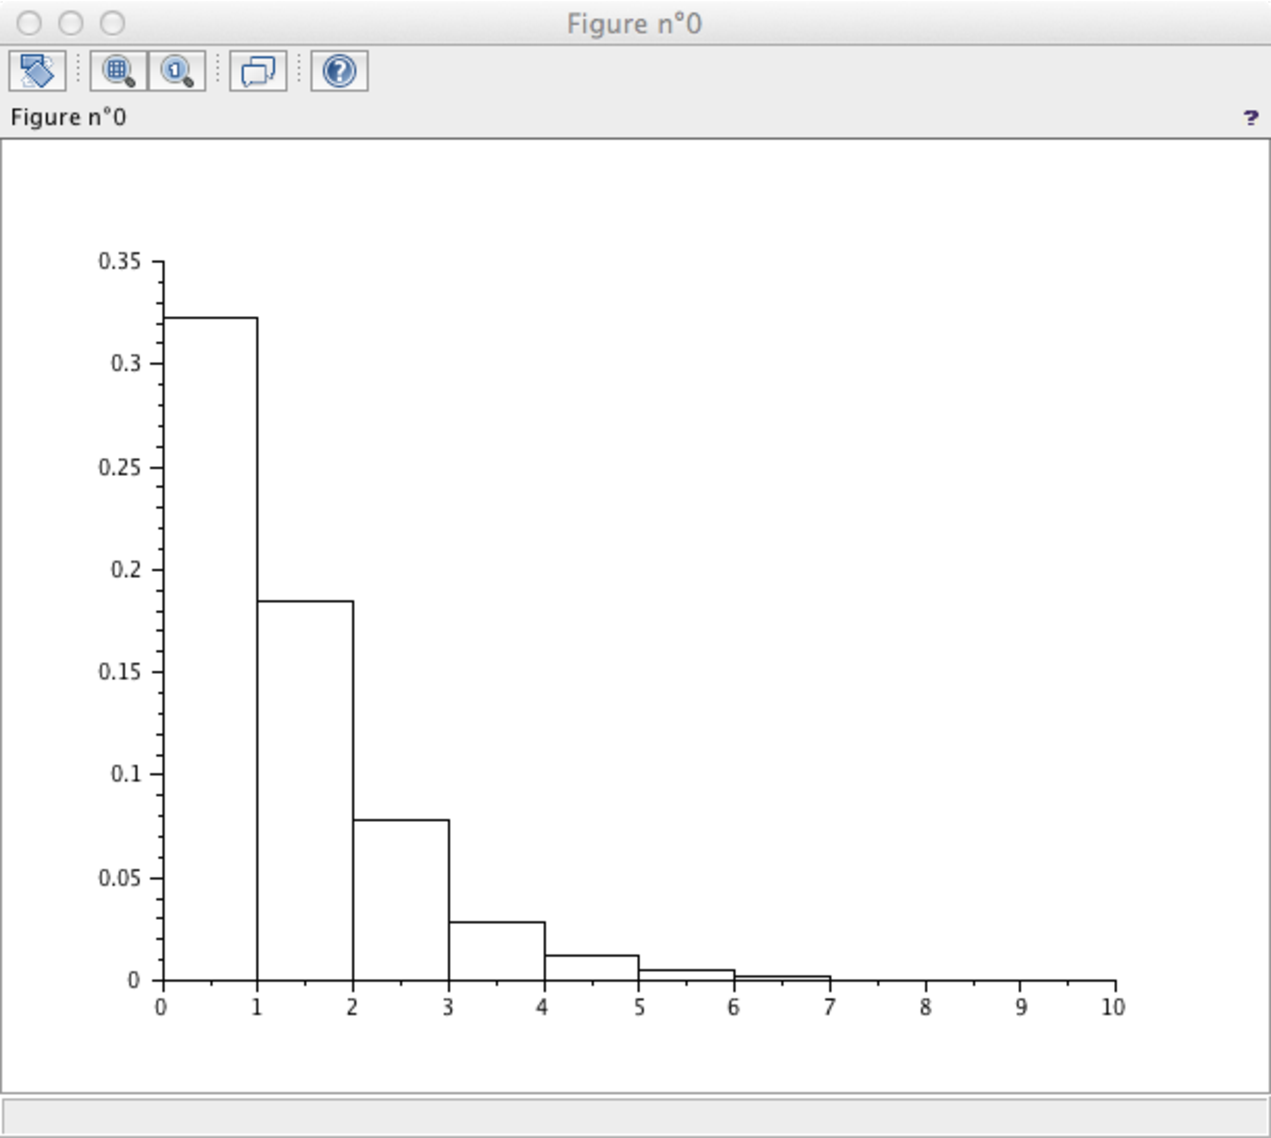
\includegraphics[width = 6cm,height =
    6cm]{Figures/EDHEC_2017/loi_faible_EDHEC_2017.pdf} & 
    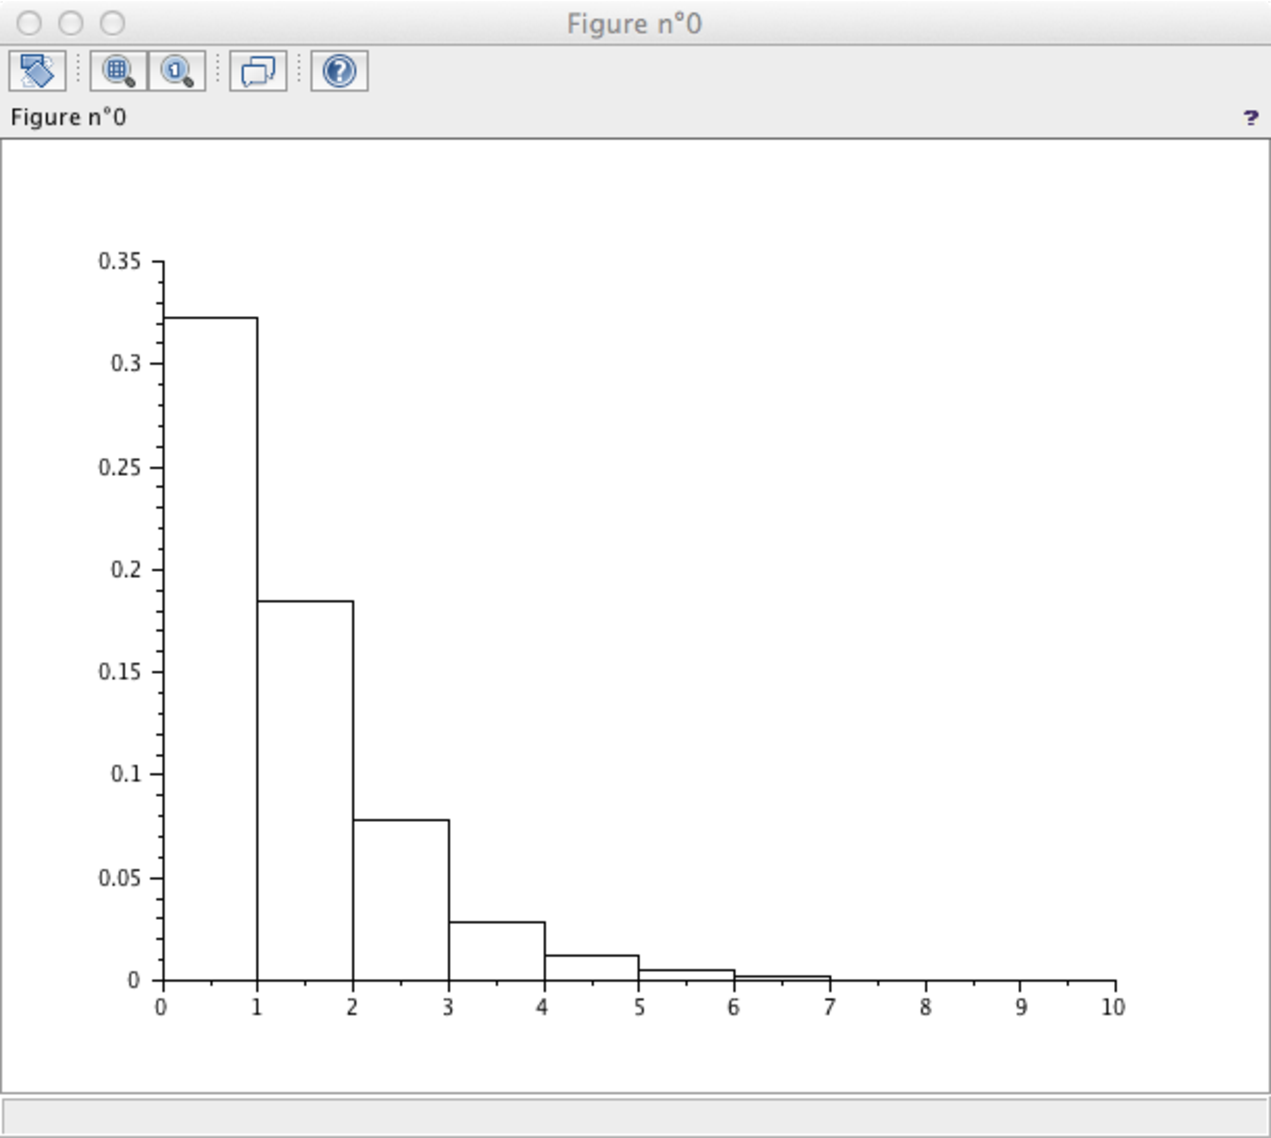
\includegraphics[width = 6cm,height =
    6cm]{Figures/EDHEC_2017/loi_faible_EDHEC_2017.pdf} \nl 
    Histogramme (1) & Histogramme (2) pour $n = 1000$
  \end{array}
  \]
  Quelle conjecture peut-on émettre quant au comportement de la suite
  des \var $(Z_{n})$ ?

  \begin{proof}~\\
    Commentons tout d'abord le script et l'histogramme $(1)$.
    \begin{noliste}{$\sbullet$}
    \item Les lignes \ligne{1} et \ligne{2} permettent d'obtenir des
      valeurs $(w_1, \ldots, w_{10000})$ qui correspondent à
      l'observation d'un $10000$-échantillon $(W_1, \ldots,
      W_{10000})$ de la \var $W$ qui suit la loi de Gumbel.\\
      (les \var $W_i$ sont indépendantes et ont même loi que $W$)
      
    \item Les lignes \ligne{3} et \ligne{4} ont pour but de permettre
      de visualiser la répartition des $10000$ valeurs $(w_1, \ldots,
      w_{10000})$ à l'aide d'un histogramme des fréquences :
      \begin{noliste}{$\stimes$}
      \item l'instruction {\tt linspace(0, 10, 11)} crée la matrice
        {\tt [0, 1, 2, \ldots, 10]}.
      \item l'instruction {\tt histplot} crée les classes : $[0,1]$,
        $]1,2]$, \ldots, $]9,10]$.\\
        Elle permet aussi de récupérer l'effectif de chaque classe
        (\ie le nombre de $w_i$ dans chaque classe) et trace
        l'histogramme $(1)$.
      \end{noliste}

    \item Considérons par exemple la classe définie par l'intervalle
      $]2, 3]$.\\
      La loi faible des grands nombres (LfGN) permet d'affirmer :
      \[
      \mbox{fréquence de la classe $]2, 3]$} = \dfrac{\mbox{effectif
          de la classe $]2, 3]$}}{\mbox{taille de l'observation}} \
      \simeq \ \Prob(\Ev{2 < W \leq 3})
      \]
      Ici, on réalise bien un grand nombre d'observations ($N =
      10000$) ce qui justifie cette formule. Ainsi, l'aire de la barre
      qui s'appuie sur l'intervalle $]2, 3]$ est donc une
      approximation de $\Prob(\Ev{2 < W \leq 3}) = F_W(3) - F_W(2)$.
    \end{noliste}
    Commentons maintenant l'histogramme $(2)$.
    \begin{noliste}{$\sbullet$}
    \item Les lignes \ligne{3}, \ligne{4}, et \ligne{5} permettent
      d'obtenir les valeurs $(u_1, \ldots, u_{10000})$ qui
      correspondent à l'observation d'un $10000$-échantillon $(U_1,
      \ldots, U_{10000})$ de la variable $Z_n$ (pour $n = 1000$).\\
      (les $U_i$ sont indépendantes et ont même loi que $Z_n$)
      
    \item On trace alors l'histogramme de répartition de ces
      valeurs. Pour les raisons évoquées ci-dessus, l'aire de la barre
      du graphique $(2)$ est une valeur approchée de :
      \[
      \Prob(\Ev{2 < Z_n \leq 3}) = F_{Z_n}(3) - F_{Z_n}(2)
      \]
    \end{noliste}%~\\


    \newpage


    \noindent
    Or, on constate que l'histogramme $(2)$ est similaire à
    l'histogramme $(1)$.\\
    Cela signifie que les aires des barres de chacun de ces deux
    graphiques sont très proches. Ainsi :
    \[   
    F_{Z_n}(3) - F_{Z_n}(2) \ \simeq \ F_{W}(3) - F_{W}(2)
    \]
    En considérant la première classe, on observe que : $F_{Z_n}(1) \
    \simeq \ F_{W}(1)$.\\
    On obtient alors, en considérant successivement toutes les classes
    :
    \[
    \forall i \in \llb 1, 10\rrb, \ F_{Z_n}(i) \ \simeq \ F_W(i)
    \]
    Les fonctions de répartition $F_{Z_n}$ et $F_{W}$ coïncident en
    ces $10$ points. En considérant des classes définies par d'autres
    points, on observerait que les fonctions coïncident en ces
    nouveaux points. Ainsi, lorsque $n = 1000$, les fonctions de
    répartition des \var $W$ et $Z_n$ sont très proches.
    % , \ie $(Z_n)$ converge en loi vers $W$. %
    \conc{On conjecture que la suite de \var $(Z_n)$ converge en loi
      vers la \var $W$.}%~\\[-1cm]
    \begin{remark}%~\\
      \begin{noliste}{$\sbullet$}
      \item Ces deux histogrammes sont normalisés. De ce fait, ce
        n'est pas l'effectif de la classe qui est affiché en ordonnée
        mais un nombre qui, une fois multiplié par la largeur de la
        barre, fournit la fréquence de la classe. Autrement dit, dans
        un tel histogramme, la fréquence d'une classe c'est l'aire de
        la barre correspondante.\\
        Ici, chaque barre est de largeur $1$. Ce sont donc les
        fréquences de chaque classe que l'on peut lire en ordonnée. Il
        ne faut pas oublier de prendre en compte ce coefficient
        multiplicatif lorsque l'on considère un nombre de barres plus
        grand (et donc des largeurs de barres différentes).
      \item Dans la démonstration, on a utilisé la loi faible des
        grands nombres (LfGN) afin de faire le lien entre fréquence de
        la classe $]2, 3]$ et probabilité $\Prob(\Ev{ 2 < W \leq 3
        })$. Établissons ce lien de manière plus précise.\\
        Pour ce faire, on introduit la \var $T$ suivante.
        \[
        \begin{array}{ccrcl}
          T & : & \Omega & \to & \R \\
          & & \omega & \mapsto & \left\{
            \begin{array}{c>{\ }R{3.4cm}}
              1 & si $W(\omega) \in \ ]2, 3]$ \nl
              0 & sinon
            \end{array}
          \right.
        \end{array}
        \]
        Le $N$-échantillon d'observations $(w_1, \ldots, w_N)$ (où $N$
        est un grand nombre) de la \var $W$ fournit un $N$-échantillon
        d'observations $(t_1, \ldots, t_N)$ de la \var $T$.\\
        La LfGN stipule :
        \[
        \dfrac{1}{N} \ \Sum{i=1}{N} t_i \ \simeq{} \ \E(T)
        \]
        Or $T$ est une \var finie qui admet pour espérance :
        \[
        \begin{array}{rcl}
          \E(T) & = & 1 \times \Prob(\Ev{2 < W \leq 3}) + \bcancel{0
            \times \Prob(\Ev{2 < W \leq 3})} \\[.2cm]
          & = & \Prob(\Ev{2 < W \leq 3}) \ = \ F_W(3) - F_W(2)
        \end{array}      
        \]
        Par ailleurs, $\Sum{i = 1}{N} t_i$ permet de compter le nombre
        d'observations qui appartiennent à la classe $]2, 3]$ (\ie
        l'effectif de la classe $]2, 3]$).\\
        Ainsi, $\frac{1}{N} \ \Sum{i = 1}{N} t_i$ est la fréquence de
        cette classe. Celle-ci est représentée graphiquement par la
        troisième barre de l'histogramme $(1)$. D'après ce qui
        précède, l'aire de cette barre est une valeur approchée de
        $\Prob(\Ev{2 < W \leq 3})$.
      \end{noliste}      
    \end{remark}~\\[-1.4cm]
  \end{proof}
\end{noliste}


\newpage


\item On note $F_{Z_{n}}$ la fonction de répartition de $Z_{n}$.
  \begin{noliste}{a)}
    \setlength{\itemsep}{2mm}
  \item Justifier que, pour tout réel $x$, on a : $F_{Z_{n}}(x) =
    F_{Y_{n}}\left(x + \ln(n)\right)$.
    
    \begin{proof}~\\
      Soit $x\in\R$.
      \[
       \begin{array}{rcl}
        F_{Z_n}(x) & = & \Prob(\Ev{Z_n \leq x})
        \\[.2cm]
        & = & \Prob(\Ev{Y_n - \ln(n) \leq x})
        \\[.2cm]
        & = & \Prob(\Ev{Y_n \leq x+\ln(n)})
        \\[.2cm]
        & = & F_{Y_n}(x+\ln(n))
       \end{array}
      \]
      \conc{$\forall x\in\R$, $F_{Z_n}(x)=F_{Y_n}(x+\ln(n))$}~\\[-1cm]
    \end{proof}

  \item Déterminer explicitement $F_{Z_{n}}(x)$.
  
  \begin{proof}~%\\
    \begin{noliste}{$\sbullet$}
    \item Déterminons tout d'abord $Z_n(\Omega)$.\\
      On a vu précédemment : $Y_n(\Omega) \subset [0, +\infty[$.%
      \conc{Comme $Z_n = Y_n - \ln(n)$, on en déduit que $Z_n(\Omega)
        \subset [-\ln(n), +\infty[$}~
    \end{noliste}
    % Or, d'après la question \itbf{6.a)},
    % $F_{Z_n}(x)=F_{Y_n}(x+\ln(n))$ et :
    % \[
    % x+\ln(n) \geq 0 \ \Leftrightarrow \ x \geq -\ln(n)
    % \]
    Déterminons $F_{Z_n}$.\\
    Soit $x\in\R$. Deux cas se présentent.
    \begin{noliste}{$\sbullet$}
    \item \dashuline{Si $x<-\ln(n)$} : alors $\Ev{Z_n \leq x} =
      \emptyset$. Ainsi :
      \[
      F_{Z_n}(x) = \Prob(\Ev{Z_n \leq x}) = \Prob(\emptyset) = 0
      \]
      % \[
      % \begin{array}{rcl@{\qquad}>{\it}R{4cm}}
      %   F_{Z_n}(x) & = & F_{Y_n}(x+\ln(n))
      %   \\[.2cm]
      %   & = & 0 & (car $x+\ln(n)<0$)
      % \end{array}
      % \]
      
      \item \dashuline{Si $x\geq -\ln(n)$}, alors :
      \[
       \begin{array}{rcl@{\qquad}>{\it}R{4cm}}
         F_{Z_n}(x) & = & F_{Y_n}(x+\ln(n))
         \\[.2cm]
         & = & \left(1-\ee^{-(x+\ln(n))}\right)^n & (car $x+\ln(n)
         \geq 0$ et par définition de $F_{Y_n}$)
         \nl[-.2cm]
         \nl
         & = & \left(1-\ee^{-x-\ln(n)}\right)^n
         \\[.4cm]
         & = & \left( 1-\ee^{-x} \ \ee^{-\ln(n)}\right)^n
         \\[.4cm]
         & = & \left(1- \ee^{-x} \ \dfrac{1}{\ee^{\ln(n)}}\right)^n
         \\[.6cm]
         & = & \left(1 - \dfrac{\ee^{-x}}{n}\right)^n
       \end{array}
      \]
    \end{noliste}
%      D'après la question \itbf{2.a)}, on sait que :
%     \[
%      F_{Y_n}(x) = \left\{
%      \begin{array}{cl}
%       0 & \mbox{ si $x<0$}\\
%       (1-\ee^{-x})^n & \mbox{ si $x\geq 0$}
%      \end{array}
%      \right.
%     \]
    \conc{$\forall x\in\R$, $F_{Z_n}(x) = \left\{
        \begin{array}{cl}
          0 & \mbox{ si $x<-\ln(n)$}\\[.2cm]
          \left(1-\dfrac{\ee^{-x}}{n}\right)^n & \mbox{ si $x\geq -\ln(n)$}
        \end{array}
      \right.$}~\\[-.8cm]
  \end{proof}
  

  \newpage


  \item Montrer que, pour tout réel $x$, on a : $ \dlim{n \to +
      \infty} n \ln\left(1-\dfrac{\ee^{-x}}{n} \right) = -\ee^{-x}$.
      
      \begin{proof}~\\
	Soit $x\in\R$.\\
	Comme $\dlim{n\to+\infty} -\dfrac{\ee^{-x}}{n}=0$, on a 
	l'équivalent suivant :
	\[
	 \ln\left(1-\dfrac{\ee^{-x}}{n}\right) \eqn -\dfrac{\ee^{-x}}{n}
	\]
	On obtient alors :
	\[
        n\ln\left(1-\dfrac{\ee^{-x}}{n}\right) \eqn
        -\bcancel{n}\dfrac{\ee^{-x}}{\bcancel{n}} = -\ee^{-x}
        \tendn -\ee^{-x}
	\]
        % De plus la quantité $-\ee^{-x}$ ne dépend pas de $n$.
	\conc{On en déduit :
          $\dlim{n\to+\infty}n\ln\left(1-\dfrac{\ee^{-x}}{n}\right) =
          -\ee^{-x}$.}~\\[-1cm]
      \end{proof}
      
  \item Démontrer le résultat conjecturé à la question \itbf{5.b)}.
  
    \begin{proof}~\\
      Il s'agit de démontrer que la suite $(Z_n)$ converge en loi vers
      la \var $W$. Autrement dit, il faut démontrer qu'en tout point
      de continuité de $F_W$, \ie pour tout $x \in \R$, on a :
      \[
      \dlim{n \tend +\infty} F_{Z_n}(x) = F_W(x)
      \]
      Soit $x\in\R$.
      \begin{noliste}{$\sbullet$}      
      \item D'après la question \itbf{6.c)},
        $\dlim{n\to+\infty}n\ln\left(1-\dfrac{\ee^{-x}}{n}\right) =
        -\ee^{-x}$.\\
        La fonction $u\mapsto \exp(u)$ étant continue sur $\R$, on a,
        par composition de limites :
        \[
        \dlim{n\to+\infty} \exp\left(n\ln 
          \left(1-\dfrac{\ee^{-x}}{n}\right)\right) = \exp 
        \left(-\ee^{-x}\right)
        \]
        \conc{$\dlim{n\to+\infty} \left(1-\dfrac{\ee^{-x}}{n}\right)^n
          = \ee^{-\ee^{-x}}$}

      \item De plus, comme le réel $x$ est fixé et que $-\ln(n) \tendn
        -\infty$, il existe un rang $n_0\in\N$ tel que :
        \[
        \forall n \geq n_0, \ x \geq -\ln(n)
        \]
        Considérons maintenant $n\geq n_0$ (ce qui est autorisé car on 
        cherche une limite quand $n$ tend vers $+\infty$). On a alors :
        \[
        F_{Z_n}(x)= \left(1-\dfrac{\ee^{-x}}{n}\right)^n \ \tendn \ 
        \ee^{-\ee^{-x}}
        \]
        On en déduit :
        \[
        \dlim{n\to+\infty} F_{Z_n}(x) = F_W(x)
        \]
      \end{noliste}
      \conc{La suite de \var $(Z_n)$ converge en loi vers la \var 
        $W$.}~\\[-1cm]
    \end{proof}
  \end{noliste}
\end{noliste}


\newpage


\section*{Problème}

\subsection*{Partie 1 : étude d'une variable aléatoire}

\noindent
Les sommets d'un carré sont numérotés 1, 2, 3, et 4 de telle façon que
les côtés du carré relient le sommet 1 au sommet 2, le sommet 2 au
sommet 3, le sommet 3 au sommet 4 et le sommet 4 au sommet 1.\\
Un mobile se déplace aléatoirement sur les sommets de ce carré selon
le protocole suivant :
\begin{noliste}{$\sbullet$}
\item Au départ, c'est à dire à l'instant $0$, le mobile est sur le
  sommet 1.
\item Lorsque le mobile est à un instant donné sur un sommet, il se
  déplace à l'instant suivant sur l'un quelconque des trois autres
  sommets, et ceci de façon équiprobable.
\end{noliste}
Pour tout $n \in \N$, on note $X_{n}$ la variable aléatoire égale au
numéro du sommet sur lequel se situe le mobile à l'instant
$n$. D'après le premier des deux points précédents, on a donc $X_{0} =
1$.
\begin{noliste}{1.}
  \setlength{\itemsep}{4mm}
\item Donner la loi de $X_{1}$, ainsi que l'espérance $\E(X_{1})$ de
  la variable $X_{1}$.

  \begin{proof}~%
    \begin{noliste}{$\sbullet$} 
    \item À l'instant $0$, le mobile se trouve sur le sommet $1$.\\
      Il peut alors se déplacer sur les sommets $2$, $3$ et $4$.%
      \conc{$X_1(\Omega) = \{2, 3, 4\}$}

    \item De plus, ce choix se fait de manière équiprobable.\\ %
      Ainsi : $\Prob(\Ev{X = 2}) = \Prob(\Ev{X = 3}) = \Prob(\Ev{X =
        4}) = \dfrac{1}{3}$.%
      \conc{On en déduit : $X_1 \suit \U{2}{4}$.}

    \item La \var $X_1$ est finie donc admet une espérance. De plus :
      \[
      \begin{array}{rcl}
        \E(X_1) & = & \Sum{k \in X_1(\Omega)}{} k \ \Prob(\Ev{X_1 =
          k})
        \\[.6cm]
        & = & 2 \ \Prob(\Ev{X_1 = 2}) + 3 \ \Prob(\Ev{X_1 = 3}) + 4 \
        \Prob(\Ev{X_1 = 4}) 
        \\[.2cm]
        & = & \dfrac{1}{3} \ (2 + 3 + 4) \ = \ \dfrac{9}{3}
        \ = \ 3
      \end{array}
      \]
      \conc{La \var $X_1$ admet une espérance donnée par : $\E(X_1) =
        3$.}
    \end{noliste}
    \begin{remark}
      \begin{noliste}{$\sbullet$}
      \item Rappelons que si $(a,b) \in \N^2$ et $a < b$, la \var $X$
        suit {\bf la loi uniforme} sur $\llb a, b \rrb$ si :
        \begin{liste}{a)}
          \setlength{\itemsep}{2mm}
          \begin{minipage}{.3\linewidth}
          \item $X(\Omega) = \llb a, b \rrb$
          \end{minipage}
          \begin{minipage}{.6\linewidth}
          \item $\forall k \in \llb a, b \rrb, \ \Prob(\Ev{X = k}) =
            \dfrac{1}{b-a+1}$
          \end{minipage}
        \end{liste}       
      \item La \var $X$ admet alors une espérance et une variance
        données par : 
        \[
        \Boxed{\E(X) = \dfrac{a+b}{2}} \quad \text{ et } \quad
        \Boxed{\V(X) = \dfrac{(b-a)(b-a+2)}{12}}
        \]
      \item Ici, $a = 2$ et $b = 4$. On retrouve bien : $\E(X_1) =
        \dfrac{2+4}{2} = \dfrac{6}{2} = 3$.
      \end{noliste}
    \end{remark}~\\[-1.4cm]
  \end{proof}
  On admet pour la suite que la loi de $X_{2}$ est donnée par :
  \[
  \Prob\left(\Ev{X_{2} = 1}\right) = \dfrac{1}{3}, \quad
  \Prob\left(\Ev{X_{2} = 2}\right) = \Prob\left(\Ev{X_{2} = 3}\right)
  = \Prob\left(\Ev{X_{2} = 4}\right) = \dfrac{2}{9}
  \]


  \newpage


\item Pour tout entier $n$ supérieur ou égal à 2, donner, en
  justifiant, l'ensemble des valeurs prises par $X_{n}$.

  \begin{proof}~\\%
    Démontrons par récurrence : $\forall n \geq 2$, $\PP{n}$ \quad
    où \quad $\PP{n}$ : $X_n(\Omega) = \llb 1, 4\rrb$.
    \begin{noliste}{\fitem}
    \item {\bf Initialisation} :\\
      D'après la question précédente, $X_1(\Omega) = \llb 2,
      4\rrb$.\\
      Trois cas se présentent alors pour le mobile à l'instant $1$ :
      \begin{noliste}{$-$}
      \item \dashuline{s'il est en position $2$} : il peut se
        retrouver en position $1$, $3$ ou $4$ à l'instant $2$.
      \item \dashuline{s'il est en position $3$} : il peut se
        retrouver en position $1$, $2$ ou $4$ à l'instant $2$.
      \item \dashuline{s'il est en position $4$} : il peut se
        retrouver en position $1$, $2$ ou $3$ à l'instant $2$.        
      \end{noliste}
      Toutes ces positions étant possibles, on obtient :
      \[
      X_2(\Omega) = \{1, 3, 4\} \cup \{1, 2, 4\} \cup \{1, 2, 3\} =
      \{1, 2, 3, 4\}
      \]
      D'où $\PP{2}$.
    \item {\bf Hérédité} : soit $n \geq 2$.\\
      Supposons $\PP{n}$ et démontrons $\PP{n+1}$ (\ie
      $X_{n+1}(\Omega) = \llb 1, 4\rrb$).\\[.2cm]
      D'après l'hypothèse de récurrence, $X_n(\Omega) = \llb 1, 4
      \rrb$. \\
      En procédant, comme dans l'étape d'initialisation, par
      disjonction de cas, on obtient :
      \[
      X_{n+1}(\Omega) = \{2, 3, 4\} \cup \{1, 3, 4\} \cup \{1, 2, 4\}
      \cup \{1, 2, 3\} = \{1, 2, 3, 4\}
      \]
      D'où $\PP{n+1}$.
    \end{noliste}
    \conc{Ainsi, par principe de récurrence : $\forall n \geq 2$,
      $\PP{n}$}
    \begin{remark}%~\\
      \begin{noliste}{$\sbullet$}
      \item Afin de déterminer formellement l'ensemble image
        $X_n(\Omega)$ d'une \var indicée par un entier $n$, il est
        classique de procéder à une récurrence. C'est une manière
        rigoureuse de présenter les choses et il faut y penser lorsque
        le résultat est donné dans l'énoncé.
      \item Ici, la question n'est pas : \og Démontrer que
        $X_n(\Omega) = \llb 1, 4 \rrb$\fg{} mais de \og donner, en
        justifiant\fg{}, $X_n(\Omega)$. La réponse n'existant pas dans
        l'énoncé, donner la réponse démontre déjà un premier niveau de
        compréhension. Dans ce cas, une démonstration moins formelle
        que la récurrence est acceptable. Ici, il s'agit
        essentiellement de dire que les $4$ sommets sont atteignables
        à l'instant $2$ et qu'il en est donc de même aux instants
        suivants.
      \end{noliste}
    \end{remark}~\\[-1.4cm]
  \end{proof}

\item
  \begin{noliste}{a)}
    \setlength{\itemsep}{2mm}
  \item Utiliser la formule des probabilités totales pour établir que,
    pour tout entier naturel $n$ supérieur ou égal à 2, on a :
    \[
    \Prob\left(\Ev{X_{n + 1} = 1}\right) =
    \dfrac{1}{3}\left(\Prob\left(\Ev{X_{n} = 2}\right) + \Prob\left(\Ev{X_{n}
          = 3}\right) + \Prob\left(\Ev{X_{n} = 4}\right)\right)
    \]

    \begin{proof}~\\%
      Soit $n \geq 2$.
      \begin{noliste}{$\sbullet$}
      \item D'après la question précédente, $X_n(\Omega) = \llb 1, 4
        \rrb$.\\
        On en déduit que $\Big( \Ev{X_n = k} \Big)_{k \in \llb 1, 4
          \rrb}$ est un système complet d'événements.

      \item Ainsi, d'après la formule de probabilités totales :
        \[
        \begin{array}{rcl@{\quad}>{\it}R{4.5cm}}
          \Prob(\Ev{X_{n+1} = 1}) & = & \Sum{k = 1}{4} \Prob(\Ev{X_n =
            k} \cap \Ev{X_{n+1} = 1})
          \\[.2cm]
          & = & \Sum{k = 1}{4} \Prob(\Ev{X_n = k}) \times
          \Prob_{\Ev{X_n = k}}(\Ev{X_{n+1} = 1}) & (si, pour tout $k
          \in \llb 1, 4\rrb$, \\ $\Prob(\Ev{X_n = k}) \neq 0$)
        \end{array}
        \]


        \newpage


      \item Or, d'après l'énoncé, pour tout $k \in \llb 1, 4\rrb$ :
        \[
        \Prob_{\Ev{X_n = k}}(\Ev{X_{n+1} = 1}) = \dfrac{1}{3} \text{
          si $k \neq 1$} \quad \text{ et } \quad \Prob_{\Ev{X_n =
            1}}(\Ev{X_{n+1} = 1}) = 0
        \]
        En effet, si l'événement $\Ev{X_n = k}$ est réalisé, c'est que
        le mobile se trouve en position $k$ à l'instant $n$.
        \begin{noliste}{$-$}
        \item Si $k \neq 1$, le mobile a alors une probabilité
          $\dfrac{1}{3}$ d'atteindre le sommet $1$ à l'instant
          suivant.
        \item Si $k = 1$, le mobile se déplace et ne peut se retrouver
          en position $1$ à l'instant suivant.
        \end{noliste}
        
      \item On en déduit :
        \[
        \begin{array}{cl@{\quad}>{\it}R{4.5cm}}
          & \Prob(\Ev{X_{n+1} = 1}) \\[.2cm]
          = & \bcancel{\Prob(\Ev{X_n = 1}) \times
            \Prob_{\Ev{X_n = 1}}(\Ev{X_{n+1} = 1})} + \Sum{k = 2}{4}
          \Prob(\Ev{X_n = k}) \times \Prob_{\Ev{X_n = k}}(\Ev{X_{n+1}
            = 1}) 
          \\[.2cm]
          = & \Sum{k = 2}{4} \Prob(\Ev{X_n = k}) \times \dfrac{1}{3}
          \ = \ \dfrac{1}{3} \ \Sum{k = 2}{4} \Prob(\Ev{X_n = k})
        \end{array}
        \]
      \end{noliste}
      \conc{$\forall n \geq 2, \ \Prob(\Ev{X_{n+1} = 1}) =
        \dfrac{1}{3} \ \Sum{k = 2}{4} \Prob(\Ev{X_n = k})$}
      \begin{remark}%~
        \begin{noliste}{$\sbullet$}
        \item Afin de pouvoir écrire $\Prob_{\Ev{X_n = k}}(\Ev{X_{n+1}
            = 1})$, il faut normalement s'assurer que $\Prob({\Ev{X_n
              = k}}) \neq 0$. Ici, l'existence de $\Prob_{\Ev{X_n =
              k}}(\Ev{X_{n+1} = 1})$ est justifiée par le paragraphe
          initial du sujet où l'on décrit la probabilité que le mobile
          se trouve en une certaine position à un instant connaissant
          sa position à l'instant précédent.
        \item La réponse est ici donnée dans l'énoncé. Il est donc
          tentant de faire de la rétro-ingénierie (partir du résultat
          pour essayer de trouver la démonstration). Ce n'est
          évidemment pas interdit mais parfois dangereux. En
          l'occurrence, on constate ici que $\Prob(\Ev{X_n = 1})$ est
          absent de la somme. La conclusion hâtive (et fausse si $n
          \geq 2$ !) est alors de déclarer que $\Big( \Ev{X_n = k}
          \Big)_{k \in \llb 2, 4 \rrb}$ est un système complet
          d'événements.
        \end{noliste}
      \end{remark}~\\[-1.4cm]
    \end{proof}

  \item Vérifier que cette relation reste valable pour $n = 0$ et $n =
    1$.

    \begin{proof}~%
      \begin{noliste}{$\sbullet$}
      \item \dashuline{Si $n = 0$} : d'après l'énoncé, le mobile se
        trouve en position $1$ à l'instant $0$. Ainsi :
        \[
        \Prob(\Ev{X_0 = 1}) = 1 \quad \text{ et } \quad \Prob(\Ev{X_0
          = 2}) = \Prob(\Ev{X_0 = 3}) = \Prob(\Ev{X_0 = 4}) = 0
        \]
        Ainsi : $\Sum{k = 2}{4} \Prob(\Ev{X_n = k}) = 0$.\\
        Comme le mobile se déplace, il ne peut se trouver en position
        $1$ à l'instant $1$ : $\Prob(\Ev{X_1 = 1}) = 0$.%
        \conc{La relation est vérifiée pour $n = 0$.}


        \newpage


      \item \dashuline{Si $n = 1$} : dans ce cas, on peut refaire la
        démonstration précédente avec le système complet d'événements
        $\Big( \Ev{X_1 = k} \Big)_{k \in \llb 1, 4 \rrb}$. La seule
        différence est que cette famille contient l'événement
        impossible $\emptyset$. D'après la formule de probabilités
        totales :
        \[
        \begin{array}{cl@{\quad}>{\it}R{5cm}}
          & \Prob(\Ev{X_{2} = 1}) 
          \\[.2cm]
          = & \Sum{k = 1}{4} \Prob(\Ev{X_1 = k} \cap \Ev{X_{2} = 1})
          \\[.4cm]
          = & \bcancel{\Prob(\Ev{X_1 = 1} \cap \Ev{X_{2} = 1})} +
          \Sum{k = 2}{4} \Prob(\Ev{X_1 = k} \cap \Ev{X_{2} = 1}) 
          & (car $\Ev{X_1 = 1} \cap \Ev{X_{2} = 1} = \emptyset$)
          \nl 
          \nl[-.4cm]
%           = & \Sum{k = 2}{4} \Prob(\Ev{X_1 = k} \cap \Ev{X_{2} = 1}) 
%           \\[.2cm]
          = & \Sum{k = 2}{4} \Prob(\Ev{X_1 = k}) \times \Prob_{\Ev{X_1
              = k}}(\Ev{X_{2} = 1}) 
          \\[.4cm]
           = & \dfrac{1}{3} \ \Sum{k = 2}{4} \Prob(\Ev{X_1 = k}) 
        \end{array}
        \]
        \conc{La relation est vérifiée pour $n = 1$.}        
      \end{noliste}
      \begin{remark}%~
        % \begin{noliste}{$\sbullet$}
        % \item
        Par définition, le système complet d'événements associé à
        $X_1$ est $\Big( \Ev{X_1 = k} \Big)_{k \in \llb 2, 4
          \rrb}$. En lui adjoignant $\Ev{X_1 = 1} = \emptyset$, la
        famille obtenue $\Big( \Ev{X_1 = k} \Big)_{k \in \llb 1, 4
          \rrb}$ est toujours un système complet d'événements. Un
        système complet d'événements n'est donc pas forcément une
        partition de l'univers $\Omega$ (les ensembles formant une
        partition sont tous non vides).
        % \end{noliste}
      \end{remark}~\\[-1.4cm]
    \end{proof}

  \item Justifier que, pour tout $n$ de $\N$, on a $\Prob(\Ev{X_{n} =
      1}) + \Prob(\Ev{X_{n} = 2}) + \Prob(\Ev{X_{n} = 3}) +
    \Prob(\Ev{X_{n} = 4}) = 1$ et en déduire l'égalité :
    \[
    \forall n \in \N, \ \Prob\left(\Ev{X_{n + 1} = 1}\right) =
    -\dfrac{1}{3} \ \Prob\left(\Ev{X_{n} = 1}\right) + \dfrac{1}{3}
    \]

    \begin{proof}~\\%
      Soit $n \in \N$.
      \begin{noliste}{$\sbullet$}
      \item La famille $\Big( \Ev{X_n = k} \Big)_{k \in \llb 1, 4
          \rrb}$ est un système complet d'événements (qui contient
        éventuellement $\emptyset$ pour les cas $n = 0$ et $n = 1$).
        On en déduit :
        \[
        \Prob(\Ev{X_{n} = 1}) + \Prob(\Ev{X_{n} = 2}) +
        \Prob(\Ev{X_{n} = 3}) + \Prob(\Ev{X_{n} = 4}) = 1
        \]

      \item Ainsi :
        \[
        \Prob(\Ev{X_{n} = 2}) + \Prob(\Ev{X_{n} = 3}) +
        \Prob(\Ev{X_{n} = 4}) = 1 - \Prob(\Ev{X_{n} = 1})
        \]
        et d'après la question précédente :
        \[
        \Prob(\Ev{X_{n+1} = 1}) = \dfrac{1}{3} \ \Sum{k = 2}{4}
        \Prob(\Ev{X_1 = k}) = \dfrac{1}{3} \ (1 - \Prob(\Ev{X_{n} =
          1}))
        \]
      \end{noliste}
      \conc{$\forall n \in \N$, $\Prob(\Ev{X_{n+1} = 1}) =
        -\dfrac{1}{3} \ \Prob(\Ev{X_n = 1}) + \dfrac{1}{3}$}~\\[-1cm]
    \end{proof}


    \newpage


  \item Établir alors que : $\forall n \in \N, \ \Prob\left(\Ev{X_{n}
        = 1}\right) = \dfrac{1}{4} +
    \dfrac{3}{4}\left(-\dfrac{1}{3}\right)^{n}$.

    \begin{proof}~\\%
      Pour tout $n\in \N$, on note : $u_n = \Prob\left(\Ev{X_{n} =
          1}\right)$.\\
      D'après la question précédente, la suite $(u_n)$ vérifie :
      \[
      \forall n \in \N, \ u_{n+1} = -\dfrac{1}{3} \ u_n + \dfrac{1}{3}
      \]
      Ainsi, $(u_n)$ est arithmético-géométrique. On lui applique la
      méthode d'étude associée.
      \begin{noliste}{$\sbullet$}
      \item L'équation de point fixe associé à la suite $(u_n)$ est :
        \[
        x = -\dfrac{1}{3} \ x + \dfrac{1}{3}
        \]
        Or : $x = -\dfrac{1}{3} \ x + \dfrac{1}{3} \ \Leftrightarrow \
        \dfrac{4}{3} \ x = \dfrac{1}{3} \ \Leftrightarrow \
        x = \dfrac{\bcancel{3}}{4} \ \dfrac{1}{\bcancel{3}}$.\\
        Ainsi, l'équation de point fixe admet pour unique solution :
        $\lambda = \dfrac{1}{4}$.\\[-.2cm]
    
      \item ~\\[-.55cm]%
        $%
        \begin{array}{rrcccccc@{\quad}>{\scriptstyle}l}
          \mbox{On écrit :} & u_{n+1} & = & -\dfrac{1}{3} & \times & 
	  u_n & + & \dfrac{1}{3} & (L_1) \\[.4cm]
          & \lambda & = & -\dfrac{1}{3} & \times & \lambda & + &
          \dfrac{1}{3} & (L_2)\\
          \\
          \mbox{et donc } & u_{n+1} - \lambda & = & -\dfrac{1}{3} & 
	  \times &
          \multicolumn{3}{l}{(u_n - \lambda)} & (L_1) - (L_2)\\
        \end{array}
        $\\[.1cm]
        Notons alors $(v_n)$ la suite de terme général $v_n = u_n -
        \lambda$.
        
     \item La suite $(v_n)$ est géométrique de raison $-\dfrac{1}{3}$.\\
        Ainsi, pour tout $n \in \N$ :
        \[
        \begin{array}{rcl}
          v_n & = & \left(-\dfrac{1}{3}\right)^{n} \times v_0 \ = \
          \left(-\dfrac{1}{3}\right)^{n} \times (u_0 - \lambda) 
          \\[.6cm]
          & = & \left(-\dfrac{1}{3}\right)^{n} \times
          \left(\Prob(\Ev{X_0 = 1}) - \dfrac{1}{4} \right)
          \\[.6cm]
          & = & \left(-\dfrac{1}{3}\right)^{n} \left(1 -
            \dfrac{1}{4}\right) \ = \ \dfrac{3}{4} \
          \left(-\dfrac{1}{3}\right)^{n} 
        \end{array}
        \]
        On a donc, pour tout $n \in \N$ :
        \[
        u_{n} \ = \ v_n + \lambda \ = \ \dfrac{3}{4} \
        \left(-\dfrac{1}{3}\right)^{n} + \dfrac{1}{4}
        \]
      \end{noliste}
      \conc{$\forall n \in \N$, $\Prob\left(\Ev{X_{n} = 1}\right) =
        \dfrac{1}{4} + \dfrac{3}{4} \
        \left(-\dfrac{1}{3}\right)^{n}$.}%~\\[-1.2cm]
      \begin{remark}%~\\
        La relation $\Prob(\Ev{X_{n+1} = 1}) = -\dfrac{1}{3} \
        \Prob(\Ev{X_n = 1}) + \dfrac{1}{3}$ (question précédente) doit
        faire penser à une suite arithmético-géométrique. Cet aspect
        est mis en évidence par l'introduction de la notation $u_n =
        \Prob\left(\Ev{X_{n} = 1}\right)$.
      \end{remark}
    \end{proof}
  \end{noliste}
  

\newpage


\item
  \begin{noliste}{a)}
    \setlength{\itemsep}{2mm}
  \item En procédant de la même façon qu'à la question précédente,
    montrer que l'on a :
    \[
    \forall n \in \N, \ \Prob\left(\Ev{X_{n + 1} = 2}\right) =
    \dfrac{1}{3} \ \left( \Prob\left(\Ev{X_{n} = 1}\right) +
      \Prob\left(\Ev{X_{n} = 3}\right) + \Prob\left(\Ev{X_{n} =
          4}\right)\right)
    \]

    \begin{proof}~\\%
      Soit $n \in \N$.
      \begin{noliste}{$\sbullet$}
      \item Si $n \geq 1$, la famille $\Big( \Ev{X_n = k} \Big)_{k \in
          \llb 1, 4 \rrb}$ est un système complet d'événements (qui
        contient $\emptyset$ si $n =1$). D'après la formule de
        probabilités totales :
        \[
        \begin{array}{cl@{\quad}>{\it}R{5.4cm}}
          & \Prob(\Ev{X_{n+1} = 2}) 
          \\[.2cm]
          = & \Sum{k = 1}{4} \Prob(\Ev{X_n = k} \cap \Ev{X_{n+1} = 2})
          \\[.2cm]
          = & \bcancel{\Prob(\Ev{X_n = 2} \cap \Ev{X_{n+1} = 2})} +
          \Sum{
            \scalebox{.8}{
              $
              \begin{array}{l}
                k = 1 \\
                k \neq 2
              \end{array}
              $
            }
          }{4} \Prob(\Ev{X_n = k} \cap \Ev{X_{n+1} = 2}) 
          & (car $\Ev{X_n = 2} \cap \Ev{X_{n+1} = 2} = \emptyset$)
          \nl 
          \nl[-.4cm]
          %\\[.2cm]
          = & \Sum{
            \scalebox{.8}{
              $
              \begin{array}{l}
                k = 1 \\
                k \neq 2
              \end{array}
              $
            }
          }{4} \Prob(\Ev{X_n = k} \cap \Ev{X_{n+1} = 2}) 
          \\[.6cm]
          = & 
          \multicolumn{2}{l}{
          \Sum{
            \scalebox{.8}{
              $
              \begin{array}{l}
                k = 1 \\
                k \neq 2
              \end{array}
              $
            }
          }{4} \Prob(\Ev{X_n = k}) \times \Prob_{\Ev{X_n =
              k}}(\Ev{X_{n+1} = 2}) \ = \ \dfrac{1}{3} \ \Sum{
            \scalebox{.8}{
              $
              \begin{array}{l}
                k = 1 \\
                k \neq 2
              \end{array}
              $
            }
          }{4} \Prob(\Ev{X_n = k})
          }
        \end{array}
        \]
        \conc{$\forall n \in \N^*$, $\Prob(\Ev{X_{n+1} = 2}) =
          \dfrac{1}{3} \ \left( \Prob\left(\Ev{X_{n} = 1}\right) +
            \Prob\left(\Ev{X_{n} = 3}\right) + \Prob\left(\Ev{X_{n} =
                4}\right)\right)$}~%

      \item Si $n = 0$, comme déjà vu :
        \[
        \Prob(\Ev{X_0 = 1}) = 1 \quad \text{ et } \quad \Prob(\Ev{X_0
          = 2}) = \Prob(\Ev{X_0 = 3}) = \Prob(\Ev{X_0 = 4}) = 0
        \]
        et $\Prob(\Ev{X_1 = 2}) = \Prob(\Ev{X_0 = 1} \cap \Ev{X_1 =
          2}) = \Prob(\Ev{X_0 = 1}) \times \Prob_{\Ev{X_0 =
            1}}(\Ev{X_1 = 2}) = 1 \times \dfrac{1}{3} = \dfrac{1}{3}$.%
        \conc{La relation est aussi vérifiée pour $n = 0$.}~\\[-1.4cm]
      \end{noliste}
    \end{proof}

  \item En déduire une relation entre $\Prob\left(\Ev{X_{n + 1} =
        2}\right)$ et $\Prob\left(\Ev{X_{n} = 2}\right)$.

    \begin{proof}~\\%
      Soit $n \in \N$.
      \begin{noliste}{$\sbullet$}
      \item Comme vu précédemment : 
        \[
        \Prob(\Ev{X_{n} = 1}) + \Prob(\Ev{X_{n} = 2}) +
        \Prob(\Ev{X_{n} = 3}) + \Prob(\Ev{X_{n} = 4}) = 1
        \]

      \item Ainsi :
        \[
        \Prob(\Ev{X_{n} = 1}) + \Prob(\Ev{X_{n} = 3}) +
        \Prob(\Ev{X_{n} = 4}) = 1 - \Prob(\Ev{X_{n} = 2})
        \]
        et d'après la question précédente :
        \[
        \Prob(\Ev{X_{n+1} = 2}) = \dfrac{1}{3} \ \Sum{ \scalebox{.8}{
            $
            \begin{array}{l}
              k = 1 \\
              k \neq 2
            \end{array}
            $ } }{4} \Prob(\Ev{X_n = k}) = \dfrac{1}{3} \ (1 -
        \Prob(\Ev{X_{n} = 2})) = - \dfrac{1}{3} \ \Prob(\Ev{X_{n} =
          2}) + \dfrac{1}{3}
        \]
      \end{noliste}
      \conc{$\forall n \in \N$, $\Prob(\Ev{X_{n+1} = 2}) = -
        \dfrac{1}{3} \ \Prob(\Ev{X_{n} = 2}) + \dfrac{1}{3}$}~\\[-1cm]
    \end{proof}


    \newpage


  \item Montrer enfin que : $\forall n \in \N, \Prob\left(\Ev{X_{n} =
        2}\right) = \dfrac{1}{4} - \dfrac{1}{4} \
    \left(-\dfrac{1}{3}\right)^{n}$.

    \begin{proof}~\\%
      Pour tout $n \in \N$, on note : $r_n = \Prob(\Ev{X_n = 2})$.\\
      D'après la question précédente, la suite $(r_n)$ vérifie :
      \[
      \forall n \in \N, \ r_{n+1} = - \dfrac{1}{3} \ r_n + \dfrac{1}{3}
      \]
      Ainsi, $(r_n)$ est arithmético-géométrique.\\
      De plus, la relation vérifiée est la même que celle vérifiée pour
      $(u_n)$.
      \begin{noliste}{$\sbullet$}
      \item En appliquant la même méthode d'étude qu'en \itbf{3.d)},
        on obtient :
        \[
        \forall n \in \N, \ w_n = \left( - \dfrac{1}{3} \right)^n
        \times (r_0 - \lambda) = \left( - \dfrac{1}{3} \right)^n
        \times \left(\Prob(\Ev{X_0 = 2}) - \dfrac{1}{4} \right) =
        -\dfrac{1}{4} \ \left( - \dfrac{1}{3} \right)^n
        \]
        où, pour tout $n \in \N$, on a posé $w_n = r_n - \lambda$.

      \item On en déduit, pour tout $n \in \N$ :
        \[
        r_n = w_n + \lambda = -\dfrac{1}{4} \ \left( - \dfrac{1}{3}
        \right)^n + \dfrac{1}{4}
        \]        
      \end{noliste}
      \conc{$\forall n \in \N$, \ $\Prob\left(\Ev{X_{n} = 2}\right) =
        \dfrac{1}{4} - \dfrac{1}{4} \ \left(-\dfrac{1}{3}\right)^{n}$}
    \begin{remark}%~\\
      \begin{noliste}{$\sbullet$}
      \item Les suites $(u_n)$ et $(r_n)$ vérifiant la même relation
        de récurrence, il n'y a pas lieu de réécrire exactement la
        même démonstration.
      \item De manière générale, si un sujet demande de réaliser, à
        détails près, deux fois la même démonstration, il faut
        détailler précisément la méthode la première fois puis
        expliquer brièvement ce qui change dans la deuxième
        démonstration.
      \end{noliste}
    \end{remark}~\\[-1.4cm]
    \end{proof}

  \end{noliste}
  
\item On admet que, pour tout entier naturel $n$, on a :
  \[
  \Prob\left(\Ev{X_{n + 1} = 3}\right) = -\dfrac{1}{3} \ 
  \Prob\left(\Ev{X_{n} = 3}\right) + \dfrac{1}{3} \quad \hbox{ et }
  \quad \Prob\left(\Ev{X_{n + 1} = 4}\right) = -\dfrac{1}{3} \ 
  \Prob\left(\Ev{X_{n} = 4}\right) + \dfrac{1}{3}
  \]
  En déduire sans calcul que :
  \[
  \forall n \in \N, \ \Prob\left(\Ev{X_{n} = 3}\right) =
  \Prob\left(\Ev{X_{n} = 4}\right) =
  \dfrac{1}{4}-\dfrac{1}{4}\left(-\dfrac{1}{3}\right)^{n}
  \]

  \begin{proof}~%
    \begin{noliste}{$\sbullet$}
    \item Pour tout $n \in \N$, on note $s_n = \Prob(\Ev{X_n = 3})$ et
      $t_n = \Prob(\Ev{X_n = 4})$.\\
      Les suites $(s_n)$ et $(t_n)$ vérifient la même relation de
      récurrence que la suite $(r_n)$.\\
      De plus, on a : $r_0 = s_0 = t_0 = 0$.
    \item On en déduit que ces suites sont égales.
    \end{noliste}
    \conc{$\forall n \in \N$, $\Prob\left(\Ev{X_{n} = 2}\right) =
      \Prob\left(\Ev{X_{n} = 3}\right) = \Prob\left(\Ev{X_{n} =
          4}\right) = \dfrac{1}{4} -\dfrac{1}{4}
      \left(-\dfrac{1}{3}\right)^{n}$}~\\[-1cm]
  \end{proof}


  \newpage

  
\item Déterminer, pour tout entier naturel $n$, l'espérance
  $\E(X_{n})$ de la variable aléatoire $X_{n}$.

  \begin{proof}~%
    \begin{noliste}{$\sbullet$}
    \item La \var $X_n$ est finie. Elle admet donc une espérance.

    \item De plus, d'après ce qui précède :
      \[
      \begin{array}{cl@{\quad}>{\it}R{3.5cm}}
        & \E(X_n) \\[.2cm]
        = & \Sum{k \in X_n(\Omega)}{} k \times
        \Prob(\Ev{X_n = k})
        \\[.4cm]
        = & \Sum{k = 1}{4} k \times \Prob(\Ev{X_n = k}) 
        % & $(\star)$
        % \nl
        % \nl[-.2cm]
        \\[.4cm]
        = & 1 \times \Prob(\Ev{X_n = 1}) + 2 \times \Prob(\Ev{X_n =
          2}) + 3 \times \Prob(\Ev{X_n = 3}) + 4 \times \Prob(\Ev{X_n
          = 4}) \qquad \quad (\star)
        \\[.2cm]
        = & \left(\dfrac{1}{4} + \dfrac{3}{4} \
          \left(-\dfrac{1}{3}\right)^{n} \right) +
        2 \times \left(\dfrac{1}{4} -\dfrac{1}{4} \
          \left(-\dfrac{1}{3}\right)^{n} \right) + 3 \times
        \left(\dfrac{1}{4} -\dfrac{1}{4} \
          \left(-\dfrac{1}{3}\right)^{n} \right) + 4 \times
        \left(\dfrac{1}{4} -\dfrac{1}{4} \
          \left(-\dfrac{1}{3}\right)^{n} \right) 
        \\[.6cm]
        = & \left(\dfrac{1}{4} + \dfrac{3}{4} \
          \left(-\dfrac{1}{3}\right)^{n} \right) +
        (2 + 3 + 4) \times \left(\dfrac{1}{4} -\dfrac{1}{4} \
          \left(-\dfrac{1}{3}\right)^{n} \right)
        \\[.6cm]
        = & \left( \dfrac{1}{4} + \dfrac{9}{4}\right) + \left(
          \dfrac{3}{4} - \dfrac{9}{4}\right) \
        \left(-\dfrac{1}{3}\right)^{n} \ = \ \dfrac{10}{4} -
        \dfrac{6}{4} \ \left(-\dfrac{1}{3}\right)^{n}
      \end{array}
      \]
      \conc{$\E(X_n) = \dfrac{5}{2} - \dfrac{3}{2} \
        \left(-\dfrac{1}{3}\right)^{n}$}~

    \item Revenons au point {\it $(\star)$}. Rigoureusement, le passage de
      la deuxième égalité à la troisième n'est valide que lorsque
      $X_n(\Omega) = \llb 1, 4 \rrb$, autrement dit pour $n \geq 2$.
      \begin{noliste}{$-$}
      \item Pour $n = 0$, $X_0(\Omega) = \{1\}$.\\
        Cependant, ajouter $k \times \Prob(\Ev{X_n = k})$ pour tout $k
        \in \llb 2, 4 \rrb$ n'a pas d'impact car toutes ces
        probabilités sont nulles.

      \item Pour $n = 1$, $X_1(\Omega) = \{2, 3, 4\}$.\\
        Cependant, ajouter $1 \times \Prob(\Ev{X_n = 1})$ n'a pas
        d'impact car cette probabilité est nulle.\\[-1.1cm]
      \end{noliste}
    \end{noliste}
  \end{proof}

\end{noliste}

\subsection*{Partie 2 : calcul des puissances d'une matrice $A$}

\noindent
Pour tout $n$ de $\N$, on considère la matrice-ligne de $\M{1,4}$ :
\[
U_{n} =
\begin{smatrix}
  \Prob\left(\Ev{X_{n} = 1}\right) & \Prob\left(\Ev{X_{n} = 2}\right)
  & \Prob\left(\Ev{X_{n} = 3}\right) & \Prob\left(\Ev{X_{n} =
      4}\right)
\end{smatrix}
\]
\begin{noliste}{1.}
  \setlength{\itemsep}{4mm}%
 \setcounter{enumi}{6}
\item 
  \begin{noliste}{a)}
    \setlength{\itemsep}{2mm}
  \item Montrer (grâce à certains résultats de la partie 1) que, si
    l'on pose $A = \dfrac{1}{3}\begin{smatrix}
      0 & 1 & 1 & 1\\
      1 & 0 & 1 & 1\\
      1 & 1 & 0 & 1\\
      1 & 1 & 1 & 0
    \end{smatrix}
    $, on a :  
    \[
    \forall n \in \N, \ U_{n + 1} = U_{n} \ A 
    \]

    \begin{proof}~\\%
      Soit $n \in \N$. Le calcul $U_n \ A$ produit une matrice ligne à
      $4$ colonnes.
      \begin{noliste}{$\sbullet$}
      \item Le coefficient de la première colonne est :
        \[
        \dfrac{1}{3} \ (\Prob(\Ev{X_n = 2}) + \Prob(\Ev{X_n = 3}) +
        \Prob(\Ev{X_n = 4}))
        \]
        D'après la question \itbf{3.a)}, ce coefficient est :
        $\Prob(\Ev{X_{n+1} = 1})$.


        \newpage


      \item Le coefficient de la deuxième colonne est :
        \[
        \dfrac{1}{3} \ (\Prob(\Ev{X_n = 1}) + \Prob(\Ev{X_n = 3}) +
        \Prob(\Ev{X_n = 4}))
        \]
        D'après la question \itbf{4.a)}, ce coefficient est :
        $\Prob(\Ev{X_{n+1} = 2})$.

      \item Les coefficients des troisième et quatrième colonnes
        sont respectivement :
        \[
        \dfrac{1}{3} \ (\Prob(\Ev{X_n = 1}) + \Prob(\Ev{X_n = 2}) +
        \Prob(\Ev{X_n = 4}))
        \]
        \[
        \dfrac{1}{3} \ (\Prob(\Ev{X_n = 1}) + \Prob(\Ev{X_n = 2}) +
        \Prob(\Ev{X_n = 3}))
        \]
        En procédant de la même manière qu'aux questions \itbf{3.a)}
        et \itbf{4.a)} (on applique la formule des probabilités
        totales avec le système complet d'événements $\Big( \Ev{X_n =
          k} \Big)_{k \in \llb 1, 4\rrb}$ pour $n \geq 1$ et on
        vérifie la formule pour $n = 0$), on reconnaît les formules
        pour :
        \[
        \Prob(\Ev{X_{n+1} = 3}) \quad \text{ et } \quad
        \Prob(\Ev{X_{n+1} = 4})
        \]
      \end{noliste}
      \conc{Finalement, on obtient bien : $\forall n \in \N$, $U_{n+1}
        = U_n \ A$.}~\\[-1cm]
    \end{proof}

  \item Établir par récurrence que : $\forall n \in \N, \ U_{n} =
    U_{0} \ A^{n}$.

    \begin{proof}~\\%
      Démontrons par récurrence : $\forall n \in \N$, $\PP{n}$
      \quad où \quad $\PP{n}$ : $U_n = U_0 \ A^n$.
      \begin{noliste}{\fitem}
      \item {\bf Initialisation} :\\
        Il suffit de remarquer : $U_0 \ A^0 = U_0 \ I = U_0$.\\
        D'où $\PP{0}$.
      \item {\bf Hérédité} : soit $n \in \N$.\\
        Supposons $\PP{n}$ et démontrons $\PP{n+1}$ (\ie $U_{n+1} =
        U_0 \ A^{n+1}$).%\\[.2cm]
        \[
        \begin{array}{rcl@{\quad}>{\it}R{3.5cm}}
          U_{n+1} & = & U_n \ A & (par définition)
          \nl
          \nl[-.2cm]
          & = & U_0 \ A^n \ A & (par hypothèse \\ de récurrence)
          \nl
          \nl[-.2cm]
          & = & U_0 \ A^{n+1}
        \end{array}
        \]
        D'où $\PP{n+1}$.
      \end{noliste}
      \conc{Ainsi, par principe de récurrence : $\forall n \in \N$,
        $\PP{n}$.}~\\[-1.2cm]
    \end{proof}

  \item En déduire la première ligne de $A^{n}$.

    \begin{proof}~\\%
      Soit $n \in \N$.
      \begin{noliste}{$\sbullet$}
      \item On récupère la première ligne de la matrice $A^n$ en la
        multipliant, à gauche, par $(1 \quad 0 \quad 0 \quad 0)$.
      \item Or : $U_0 = (\Prob(\Ev{X_0 = 1}) \quad \Prob(\Ev{X_0 = 2})
        \quad \Prob(\Ev{X_0 = 3}) \quad \Prob(\Ev{X_0 = 4})) = (1
        \quad 0 \quad 0 \quad 0)$.
      \item D'après la question précédente, $U_n = U_0 \ A^n$.\\
        Ainsi, la première ligne de $A^n$ n'est autre que $U_n$.%
        \concL{La première ligne de $A^n$ est $U_n = (\Prob(\Ev{X_n =
            1}) \quad \Prob(\Ev{X_n = 2}) \quad \Prob(\Ev{X_n = 3})
          \quad \Prob(\Ev{X_n = 4}))$, à savoir : \\[.2cm]
          $\left( \dfrac{1}{4} + \dfrac{3}{4} \ \left(
              -\dfrac{1}{3}\right)^n \quad \dfrac{1}{4} - \dfrac{1}{4}
            \ \left( -\dfrac{1}{3}\right)^n \quad \dfrac{1}{4} -
            \dfrac{1}{4} \ \left( -\dfrac{1}{3}\right)^n \quad
            \dfrac{1}{4} - \dfrac{1}{4} \ \left(
              -\dfrac{1}{3}\right)^n \right)$.}{14}~\\[-1.2cm]
      \end{noliste}
    \end{proof}
  \end{noliste}
  
  
  \newpage
  
  
\item Expliquer comment choisir la position du mobile au départ pour
  trouver les trois autres lignes de la matrice $A^{n}$, puis écrire
  ces trois lignes.

  \begin{proof}~%
    \begin{noliste}{$\sbullet$}
    \item On récupère la deuxième ligne de la matrice $A^n$ en la
      multipliant, à gauche, par $(0 \quad 1 \quad 0 \quad 0)$.\\
      Il faut donc considérer : 
      \[
      U_0 = (\Prob(\Ev{X_0 = 1}) \quad \Prob(\Ev{X_0 = 2}) \quad
      \Prob(\Ev{X_0 = 3}) \quad \Prob(\Ev{X_0 = 4})) = (0 \quad 1
      \quad 0 \quad 0)
      \]
      ce qui signifie que $\Prob(\Ev{X_0 = 2}) = 1$.%
      \concL{En plaçant le mobile initialement en position $2$, la
        multiplication $U_0 \ A^n$ permet de récupérer la deuxième
        ligne de $A^n$.}{14}%
      \concL{De même, on récupère la troisième ligne de $A^n$ en
        considérant $(0 \quad 0 \quad 1 \quad 0)$, ce qui correspond à
        placer initialement le mobile en position $3$.}{14}%
      \concL{Enfin, on récupère la quatrième ligne de $A^n$ en
        considérant $(0 \quad 0 \quad 0 \quad 1)$, ce qui correspond à
        placer initialement le mobile en position $4$.}{14}
    \item Ces choix modifient les calculs faits en question
      \itbf{3.d)}, \itbf{4.c)} et \itbf{5}.\\
      Plus précisément, cela modifie les valeurs initiales des suites
      $(u_n)$, $(r_n)$, $(s_n)$ et $(t_n)$.\\
      Par exemple, pour le choix $U_0 = (0 \quad 1 \quad 0 \quad 0)$,
      on obtient :
      \[
      u_0 = 0 \qquad r_0 = 1 \qquad s_0 = 0 \qquad t_0 = 0
      \]
      Chacune de ces suites vérifie la même relation de
      récurrence.\\
      Seule la condition initiale (premier terme nul ou égal à $1$)
      les différencie.
      \begin{noliste}{$-$}
      \item La question \itbf{3.d)} nous fournit le terme général pour
        une valeur initiale nulle.
      \item La question \itbf{4.c)} nous fournit le terme général pour
        une condition initiale égale à $1$.
      \end{noliste}
      \concL{La deuxième ligne de $A^n$ est : \\[.2cm]
        $\left( \dfrac{1}{4} - \dfrac{1}{4} \ \left(
            -\dfrac{1}{3}\right)^n \quad \dfrac{1}{4} + \dfrac{3}{4} \
          \left( -\dfrac{1}{3}\right)^n \quad \dfrac{1}{4} -
          \dfrac{1}{4} \ \left( -\dfrac{1}{3}\right)^n \quad
          \dfrac{1}{4} - \dfrac{1}{4} \ \left( -\dfrac{1}{3}\right)^n
        \right)$}{14}%
      \concL{La troisième ligne de $A^n$ est : \\[.2cm]
        $\left( \dfrac{1}{4} - \dfrac{1}{4} \ \left(
            -\dfrac{1}{3}\right)^n \quad \dfrac{1}{4} - \dfrac{1}{4} \
          \left( -\dfrac{1}{3}\right)^n \quad \dfrac{1}{4} +
          \dfrac{3}{4} \ \left( -\dfrac{1}{3}\right)^n \quad
          \dfrac{1}{4} - \dfrac{1}{4} \ \left( -\dfrac{1}{3}\right)^n
        \right)$}{14}
      \concL{La quatrième ligne de $A^n$ est : \\[.2cm]
        $\left( \dfrac{1}{4} - \dfrac{1}{4} \ \left(
            -\dfrac{1}{3}\right)^n \quad \dfrac{1}{4} - \dfrac{1}{4} \
          \left( -\dfrac{1}{3}\right)^n \quad \dfrac{1}{4} -
          \dfrac{1}{4} \ \left( -\dfrac{1}{3}\right)^n \quad
          \dfrac{1}{4} + \dfrac{3}{4} \ \left( -\dfrac{1}{3}\right)^n
        \right)$}{14}~\\[-1cm]
    \end{noliste}
  \end{proof}
\end{noliste}

% \begin{remark}%~
%   \begin{noliste}{$\sbullet$}
%   \item On peut généraliser la méthode abordée dans les questions
%     \itbf{7.c)} et \itbf{7.d)}. 
%     \[
%     (x \quad y \quad z \quad t) \ A = x \cdot L_1 + y \cdot L_2 + z
%     \cdot L_3 + z \cdot L_4
%     \]
%     où $L_1$, $L_2$, $L_3$, $L_4$ sont les lignes de $A$.\\
%     On retiendra qu'en multipliant à gauche, on agit sur les lignes.
%   \item De même :
%     \[
%     A \
%     \begin{smatrix}
%       x \\
%       y \\
%       z \\
%       t
%     \end{smatrix}
%     = x \cdot C_1 + y \cdot C_2 + z \cdot C_3 + z \cdot C_4
%     \]
%     où $C_1$, $C_2$, $C_3$, $C_4$ sont les colonnes de $A$.\\
%     On retiendra qu'en multipliant à gauche, on agit sur les colonnes.
%   \end{noliste}

% \end{remark}


\newpage


\subsection*{Partie 3 : une deuxième méthode de calcul des puissances
  de $A$}

\noindent
On considère les matrices $I$ et $J$ suivantes : $I =
\begin{smatrix}
  1 & 0 & 0 & 0\\
  0 & 1 & 0 & 0\\
  0 & 0 & 1 & 0\\
  0 & 0 & 0 & 1
\end{smatrix}
$ et $J = 
\begin{smatrix}
  1 & 1 & 1 & 1\\
  1 & 1 & 1 & 1\\
  1 & 1 & 1 & 1\\
  1 & 1 & 1 & 1
\end{smatrix}
$.
\begin{noliste}{1.}
  \setlength{\itemsep}{4mm}%
  \setcounter{enumi}{8}
\item Déterminer les réels $a$ et $b$ tels que $A = aI + bJ$.

  \begin{proof}~\\%
    Soit $(a, b) \in \R^2$.\\
    On a alors :
    \[
    \begin{array}{rcl}
      a \ I + b \ J = A & \Longleftrightarrow & 
      \begin{smatrix}
        a + b & b & b & b \\[.1cm]
        b & a + b & b & b \\[.1cm]
        b & b & a + b & b \\[.1cm]
        b & b & b & a + b
      \end{smatrix}
      =
      \begin{smatrix}
        0 & \frac{1}{3} & \frac{1}{3} & \frac{1}{3} \\[.1cm]
        \frac{1}{3} & 0 & \frac{1}{3} & \frac{1}{3} \\[.1cm]
        \frac{1}{3} & \frac{1}{3} & 0 & \frac{1}{3} \\[.1cm]
        \frac{1}{3} & \frac{1}{3} & \frac{1}{3} & 0
      \end{smatrix}
      \\[1cm]
      & \Longleftrightarrow & 
      \left\{
        \begin{array}{rcrcr}
          a & + & b & = & 0 \\
          & & b & = & \frac{1}{3}
        \end{array}
      \right.
      \\[.6cm]
      & 
      \begin{arrayEq}
        L_1 \leftarrow L_1 - L_2
      \end{arrayEq}
      & 
      \left\{
        \begin{array}{rcrcr}
          a & & & = & -\frac{1}{3} \\
          & & b & = & \frac{1}{3}
        \end{array}
      \right.
    \end{array}
    \]
    \conc{$A = -\frac{1}{3} \ I + \frac{1}{3} \ J$}%~\\[-1cm]
    \begin{remark}%~
      \begin{noliste}{$\sbullet$}
      \item Il est assez classique (c'est le cas ici) que les
        premières questions d'une nouvelle partie soient très
        abordables. Il est conseillé de repérer ces questions au début
        de l'épreuve en passant quelques minutes à cocher les
        questions qui semblent les plus simples.\\
        On peut citer parmi celles-ci (liste non exhaustive) :
        \begin{noliste}{$-$}
        \item l'étude du problème pour des petites valeurs d'un
          paramètre considéré (question \itbf{1.}),
        \item du calcul (questions \itbf{7.a)}, \itbf{9.} et
          \itbf{10.a)}), des applications numériques, vérifier qu'une
          relation est vraie pour certaines valeurs d'un paramètre
          (question \itbf{3.b)}),
        \item les questions dont l'énoncé souffle la méthode à
          utiliser (questions \itbf{3.a)} et \itbf{10.b)}),
        \item les méthodes / questions classiques (questions
          \itbf{3.d)} et \itbf{7.b)}).
        \end{noliste}
        L'objectif est de ne pas sortir de la salle sans avoir traité
        ces questions. Il faut donc gérer son temps en conséquence.
      \item On retiendra que les questions d'un énoncé ne sont pas
        rangées dans un ordre croissant de difficulté. Il ne faut donc
        pas se décourager si on ne sait pas traiter une ou plusieurs
        questions d'affilée. Il faut au contraire s'accrocher : des
        questions plus simples apparaîtront.
      \end{noliste}
    \end{remark}~\\[-1.2cm]
  \end{proof}

\item
  \begin{noliste}{a)}
    \setlength{\itemsep}{2mm}
  \item Calculer $J^{2}$ puis établir que, pour tout entier naturel
    $k$ non nul, on a : $J^{k} = 4^{k-1} J$.

    \begin{proof}~%
      \begin{noliste}{$\sbullet$}
      \item Tout d'abord : %
        \conc{%
          $ J^2 =
          \begin{smatrix}
            1 & 1 & 1 & 1 \\
            1 & 1 & 1 & 1 \\
            1 & 1 & 1 & 1 \\
            1 & 1 & 1 & 1
          \end{smatrix}
          \begin{smatrix}
            1 & 1 & 1 & 1 \\ 
            1 & 1 & 1 & 1 \\ 
            1 & 1 & 1 & 1 \\ 
            1 & 1 & 1 & 1 
          \end{smatrix}
          =
          \begin{smatrix}
            4 & 4 & 4 & 4 \\ 
            4 & 4 & 4 & 4 \\ 
            4 & 4 & 4 & 4 \\ 
            4 & 4 & 4 & 4 
          \end{smatrix}
          = 
          4 \cdot J
          $}
        

        \newpage


      \item Démontrons par récurrence : $\forall k \in \N^*$,
        $\PP{k}$ \quad où \quad $\PP{k}$ : $J^k = 4^{k-1} \ J$.
        \begin{noliste}{\fitem}
        \item {\bf Initialisation} :\\
          D'une part : $J^1 = J$.\\
          D'autre part : $4^{1-1} \ J = 4^0 \ J = J$.\\[.1cm]
          D'où $\PP{1}$.
        \item {\bf Hérédité} : soit $k \in \N^*$.\\
          Supposons $\PP{k}$ et démontrons $\PP{k+1}$ (\ie $J^{k+1} =
          4^k \ J$).
          \[
          \begin{array}{rcl@{\quad}>{\it}R{3.5cm}}
            J^{k+1} & = & J^k \ J \\[.2cm]
            & = & 4^{k-1} \ J \ J & (par hypothèse \\ de récurrence)
            \nl 
            \nl[-.2cm]
            & = & 4^{k-1} \ J^2
            \\[.2cm]
            & = & 4^{k-1} \ (4 \ J) \ = \ 4^k \ J
          \end{array}
          \]
          D'où $\PP{k+1}$.
        \end{noliste}
        \conc{Ainsi, par principe de récurrence : $\forall k \in
          \N^*$, $\PP{k}$.}~\\[-1.5cm]
      \end{noliste}
    \end{proof}

  \item À l'aide de la formule du binôme de Newton, en déduire, pour
    tout entier $n$ non nul, l'expression de $A^{n}$ comme combinaison
    linéaire de $I$ et $J$.

    \begin{proof}~\\%
      Soit $n \in \N^*$.
      \begin{noliste}{$\sbullet$}
      \item Les matrices $-\frac{1}{3} \ I$ et $\frac{1}{3} \ J$
        commutent puisque $I$ commute avec toute matrice carrée de
        même ordre.

      \item Par la formule du binôme de Newton :
        \[
        \begin{array}{rcl@{\quad}>{\it}R{4cm}}
          \left(-\dfrac{1}{3} \ I + \dfrac{1}{3} \ J\right)^n & = &
          \Sum{k = 0}{n} \dbinom{n}{k} \left( -\dfrac{1}{3} \ I
          \right)^{n-k} \ \left( \dfrac{1}{3} \ J \right)^{k} 
          \\[.6cm]
          & = & 
          \Sum{k = 0}{n} \dbinom{n}{k} \left( -\dfrac{1}{3}
          \right)^{n-k} \ I^{n-k} \ \left( \dfrac{1}{3} \right)^{k}  \ J^k
          \\[.6cm]
          & = & 
          \Sum{k = 0}{n} \dbinom{n}{k} (-1)^{n-k} \left(\dfrac{1}{3}
          \right)^{n-k} \ \left( \dfrac{1}{3} \right)^{k} \ I^{n-k} \ J^k
          \\[.6cm]
          & = & 
          \Sum{k = 0}{n} \dbinom{n}{k} (-1)^{n-k} \left(\dfrac{1}{3}
          \right)^{n} \ J^k & ($I^{n-k} \ J^k = I \ J^k = J^k$)
          \nl 
          \nl[-.2cm]
          & = & 
          \left(\dfrac{1}{3} \right)^{n} \ \Sum{k = 0}{n}
          \dbinom{n}{k} (-1)^{n-k} \ J^k
          \\[.6cm]
          & = & 
          \left(\dfrac{1}{3} \right)^{n} \ \left( \dbinom{n}{0} (-1)^n
            J^0 \ + \ \Sum{k = 1}{n} \dbinom{n}{k} (-1)^{n-k} \ J^k
          \right)
          & (ce découpage est \\ valable car $n \geq 0$)
          \nl 
          \nl[-.2cm]
          & = & 
          \left(\dfrac{1}{3} \right)^{n} \ \left( (-1)^n \ I \ + \
            \Sum{k = 1}{n} \dbinom{n}{k} (-1)^{n-k} \ 4^{k-1} \ J
          \right)
          & (car $J^k = 4^{k-1} \ J$ \\ pour $k \geq 1$)
          \nl 
          \nl[-.2cm]
          & = & 
          \left(\dfrac{1}{3} \right)^{n} \ \left( (-1)^n \ I \ + \
            \dfrac{1}{4} \ \left( \Sum{k = 1}{n} \dbinom{n}{k}
              (-1)^{n-k} \ 4^{k} \right) \ J \right)
        \end{array}
        \]


        \newpage


      \item Or :
        \[
        \begin{array}{rcl}
          \Sum{k = 1}{n} \dbinom{n}{k} (-1)^{n-k} \ 4^{k} & = &
          \left( \Sum{k = 0}{n} \dbinom{n}{k} (-1)^{n-k} \ 4^{k} \right) - 
          \dbinom{n}{0} (-1)^{n} \ 4^{0}
          \\[.4cm]
          & = & 
          \left( -1 + 4 \right)^n - (-1)^{n} \ = \ 3^n - (-1)^n
        \end{array}
        \]

      \item En réinjectant, on obtient :
        \[
        \begin{array}{rcl@{\quad}>{\it}R{4cm}}
          \left(-\dfrac{1}{3} \ I + \dfrac{1}{3} \ J\right)^n & = &
          \left(\dfrac{1}{3} \right)^{n} \ \left( (-1)^n \ I \ + \
            \dfrac{1}{4} \ \left( 3^n - (-1)^n \right) \ J \right)
          \\[.6cm]
          & = & \left(-\dfrac{1}{3} \right)^{n} \ I + \dfrac{1}{4} \
          \left( 1 - \left(-\dfrac{1}{3} \right)^{n} \right) \ J  
        \end{array}
        \]
        \conc{$\forall n \in \N^*$, $A^n = \left(-\dfrac{1}{3}
          \right)^{n} \ I + \dfrac{1}{4} \ \left( 1 -
            \left(-\dfrac{1}{3} \right)^{n} \right) \ J$}
      \end{noliste}
      \begin{remark}%~
        \begin{noliste}{$\sbullet$}
        \item La relation de Chasles stipule que pour tout $(m, p, n)
          \in \N^3$ tel que $m \leq p \leq n$ :
          \[
          \Sum{k = m}{n} u_k = \Sum{k = m}{p} u_k + \Sum{k = p+1}{n}
          u_k
          \]
          {\it (la deuxième somme est nulle si $p = n$)}\\
          où $(u_n)$ est une suite quelconque de réels ou de
          matrices.
          % On insiste ici sur le fait que cette relation n'est
          % vérifiée que sous la condition $m \leq p \leq n$.
        \item Dans cette question, on est dans le cas où $m = 0$ et $p
          = 0$.\\
          L'argument $n \geq 0$ est donc suffisant pour découper la
          somme. On traite le cas $n \geq 1$ dans cette question pour
          s'assurer que la deuxième somme ne se fait pas sur un
          ensemble d'indices vide. Ceci permet d'assurer que $k$ est
          et donc d'utiliser l'égalité : $J^k = 4^{k-1} \ J$.
        \end{noliste}
      \end{remark}~\\[-1.2cm]
    \end{proof}

  \item Vérifier que l'expression trouvée reste valable pour $n = 0$.

    \begin{proof}~%\\%
      \begin{noliste}{$\sbullet$}
      \item D'une part : $A^0 = I$.
      \item D'autre part : $\left(-\dfrac{1}{3} \right)^{0} \ I +
        \dfrac{1}{4} \ \left( 1 - \left(-\dfrac{1}{3} \right)^{0}
        \right) \ J \ = \ I + \dfrac{1}{4} (1 - 1) \ J \ = \ I$.
      \end{noliste}
      \conc{La relation précédente est valable pour $n = 0$.}~\\[-1.2cm]
    \end{proof}
  \end{noliste}
\end{noliste}

\subsection*{Partie 4 : informatique}

\begin{noliste}{1.}
  \setlength{\itemsep}{4mm}%
  \setcounter{enumi}{10}
\item
  \begin{noliste}{a)}
    \setlength{\itemsep}{2mm}
  \item Compléter le script \Scilab{} suivant pour qu'il affiche les
    100 premières positions autres que celle d'origine, du mobile dont
    le voyage est étudié dans ce problème, ainsi que le nombre $n$ de
    fois où il est revenu sur le sommet numéroté 1 au cours de ses 100
    premiers déplacements (on pourra utiliser la commande {\tt sum}).
    \begin{scilab}
      & A = [------] / 3 \nl %
      & x = grand(100,\ttq{}markov\ttq{},A,1) \nl %
      & n = ------ \nl %
      & disp(x) \nl %
      & disp(n) \nl %
    \end{scilab}


    \newpage


    \begin{proof}~%
      \begin{noliste}{$\sbullet$}
      \item On commence par écrire la matrice $A$.
        \begin{scilab}
          & A = [0, 1, 1, 1; 1, 0, 1, 1; 1, 1, 0, 1; 1, 1, 1, 0] / 3
        \end{scilab}

      \item La commande {\tt grand(100,\ttq{}markov\ttq{},A,1)}
        renvoie une trajectoire possible du mobile de taille
        $100$. C'est une matrice ligne $[x_1, \ldots, x_{100}]$ où les
        éléments $x_1 \in X_1(\Omega)$, \ldots, $x_{100} \in
        X_{100}(\Omega)$ sont des sommets visités par le mobile dans
        un parcours de taille $100$.\\
        Cette matrice est stockée dans la variable {\tt x}.

      \item On complète le deuxième trou du programme par
        l'instruction :
        \begin{scilabC}{2}
          & n = sum(x == 1)
        \end{scilabC}
        Détaillons brièvement :
        \begin{noliste}{$-$}
        \item l'instruction {\tt x == 1} est un test d'égalité
          effectué terme à terme.\\
          Plus précisément, cette commande permet le calcul de la
          matrice ligne de taille $100$ correspondant à :
          \[
          [x_1 == 1, \ldots, x_{100} == 1]
          \]
          {\it (on teste si chaque élément de la matrice {\tt x} vaut
            $1$)}\\
          Le résultat obtenu est une matrice ligne de booléens.
          
        \item la commande {\tt sum} permet de sommer tous les éléments
          de la matrice ligne de booléens précédents. Lors de cette
          somme, les booléens {\tt True} sont convertis en l'entier
          $1$ et les booléens {\tt False} sont convertis en l'entier
          $0$. Ainsi, {\tt sum(x == 1)} permet de compter le nombre de
          coefficients qui sont égaux à $1$ de la matrice {\tt x}.
        \end{noliste}
      \end{noliste}
      \begin{remark}%~\\
        \begin{noliste}{$\sbullet$}
        \item Un tel niveau d'explication n'est pas attendu aux
          concours : l'écriture des lignes manquantes démontre la
          compréhension de toutes les commandes en question.\\
          On décrit ici de manière précise les instructions afin
          d'aider le lecteur un peu moins habile en \Scilab{}.
        \item La ligne \ligne{3} est une manière de procéder
          spécifique à \Scilab{}.\\
          On tire notamment profit de tous les outils prédéfinis du
          langage permettant la manipulation simple et efficace (en
          temps de calcul) de matrices, qui, rappelons-le, est l'objet
          de base de ce langage.
        \item Cependant, on pouvait opter pour une version plus
          générale, pouvant s'adapter plus facilement aux autres
          langages. Pour ce faire, on remplace la ligne \ligne{3} par
          les instructions suivantes :
          \begin{scilabC}{2}
            & n = 0 \nl %
            & \tcFor{for} i = 1:100 \nl%
            & \qquad \tcIf{if} x(i) == 1 then \nl %
            & \qquad \qquad n = n+1 \nl %
            & \qquad \tcIf{end} \nl %
            & \tcIf{end}
          \end{scilabC}
          Ces instructions permettent, à l'aide d'une structure
          itérative (boucle {\tt for}) de tester un à un les éléments
          de {\tt x}. Si le coefficient testé vaut $1$, on incrémente
          un compteur {\tt n} initialisé à $0$. Ainsi, on
          compte le nombre d'éléments de {\tt x} qui sont égaux à $1$.\\
          Cette version, bien que moins idiomatique, est évidemment
          acceptée aux concours.
        \end{noliste}
      \end{remark}
    \end{proof}


    \newpage


  \item Après avoir exécuté cinq fois ce script, les réponses
    concernant le nombre de fois où le mobile est revenu sur le sommet
    1 sont : $n = 23$, $n = 28$, $n = 23$, $n = 25$, $n = 26$.\\
    En quoi est-ce normal ?

    \begin{proof}~%\\%
      \begin{noliste}{$\sbullet$}
      \item Pour tout $n \in \N$, notons $Y_n$ la \var définie par :
        \[
        Y_n =
        \left\{
        \begin{array}{cR{2cm}}
          1 & si $X_n = 1$ 
          \nl
          %\nl[-.2cm]
          0 & si $X_n \neq 1$
        \end{array}
        \right.
        \]
        La \var $Y_n$ suit une loi de Bernoulli de paramètre $p_n =
        \Prob(\Ev{X_n = 1}) = \dfrac{1}{4} + \dfrac{3}{4} \
        \left(-\dfrac{1}{3}\right)^n$.

      \item On remarque alors :
        \begin{noliste}{$-$}
        \item pour $n = 1$, $p_0 = 0$,
        \item pour $n \geq 2$, $p_n \simeq \dfrac{1}{4}$. En effet :
          \[
          \begin{array}{rcccccccr}
            \dfrac{3}{4} \ \left(-\dfrac{1}{3}\right)^2 & = &
            \dfrac{3}{4} \ \dfrac{1}{3^2} & = & \dfrac{1}{12} & \simeq &
            \dfrac{1}{10} & = & 0,1
            \\[.6cm]
            \dfrac{3}{4} \ \left(-\dfrac{1}{3}\right)^3 & = &
            \dfrac{3}{4} \ \dfrac{-1}{3^3} & = & -\dfrac{1}{36} & \simeq &
            -\dfrac{3}{100} & = & -0,03
            \\[.6cm]
            \dfrac{3}{4} \ \left(-\dfrac{1}{3}\right)^4 & = &
            \dfrac{3}{4} \ \dfrac{1}{3^4} & = & -\dfrac{1}{108} & \simeq &
            \dfrac{1}{100} & = & 0,01
          \end{array}
          \]
          et pour $n \geq 5$, $\left| \dfrac{3}{4} \
            \left(-\dfrac{1}{3}\right)^n \right| = \dfrac{1}{4 \
            3^{n-1}} < 0,01$.          
        \end{noliste}
        Ainsi, pour $n \geq 2$, on peut considérer que $Y_n \suit
        \Bern{\frac{1}{4}}$ et que $(Y_2, \ldots, Y_{100})$ est un
        $99$-échantillon d'une \var $Y$ qui suit la loi de Bernoulli
        de paramètre $\frac{1}{4}$.

      \item La matrice obtenue par l'instruction {\tt x == 1} est une
        simulation informatique de cet échantillon.\\
        Autrement dit, cette matrice s'écrit $[y_2, \ldots, y_{100}]$
        où, pour tout $i \in \llb 2, 100\rrb$, $y_i \in Y_i(\Omega)$.\\[.2cm]
        En vertu de la loi (faible) des grands nombres :
        \[
        \dfrac{1}{99} \ \Sum{k=2}{100} y_k \ \simeq \ \E(Y) =
        \Prob(\Ev{Y = 1}) = \dfrac{1}{4} \quad \text{ et ainsi } \quad
        \Sum{k=2}{100} y_k \ \simeq \ \dfrac{99}{4} \simeq 25
        \]       

      \item On conclut en remarquant que $\Sum{k=1}{100} y_k =
        \Sum{k=2}{100} y_k$ car $y_1 = 0$ ($Y_1$ est constante égale à
        $0$).
      \end{noliste}
      \conc{Il est donc normal que le mobile revienne environ $25$
        fois en position $1$.}
      % À chaque fois que $100$ déplacements sont effectués, on note
      % environ $25$ retours en position $1$. Cela correspond à la
      % formule obtenue précédemment :
      % \[
      % \Prob(\Ev{X_m = 1}) = \dfrac{1}{4} + \dfrac{3}{4} \
      % \left(-\dfrac{1}{3}\right)^m
      % \]
      % avec $\left(-\dfrac{1}{3}\right)^m$ qui se rapproche rapidement
      % de $0$.
      \begin{remark}%~\\
        \begin{noliste}{$\sbullet$}
        \item Nous avons essayé ici de formaliser la réponse à cette
          question. Cependant, la formulation de la question (\og En
          quoi est-ce normal ? \fg{}) laisse penser qu'une
          démonstration moins formelle serait acceptée.
        \item L'idée est alors de dire qu'à chaque étape (hormis la
          $\ere{1}$), le mobile a environ $1$ chance sur $4$ de se
          retrouver en position $1$. Donc en $99$ étapes, il est passé
          par la position $1$ environ $99 \times \dfrac{1}{4} \simeq
          25$ fois.
        \end{noliste}
      \end{remark}~\\[-1.4cm]
    \end{proof}
  \end{noliste}
\end{noliste}


\newpage


\begin{remark}
  \begin{noliste}{$\sbullet$}
  \item Le problème traite de l'évolution d'une grandeur aléatoire qui
    varie dans le temps discret. Plus précisément, il s'agit ici de la
    position du mobile (notée $X_n$ à l'instant $n$) sur les sommets
    d'un carré. Cette évolution se fait selon un schéma classique en
    mathématiques : le futur (\ie la valeur de $X_{n+1}$, position du
    mobile à l'instant $n+1$) ne dépend du passé (position du mobile
    aux instants précédents) que par le présent (\ie la valeur de
    $X_{n}$, position du mobile à l'instant $n$). On dit alors que
    $(X_n)$ est une {\bf chaîne de Markov}.
  \item L'évolution de la position de l'instant $n$ à l'instant $n+1$
    peut être représenté par le schéma suivant.\\[-1.8cm]
    \begin{center}
      \scalebox{.8}{$
      \begin{tikzpicture}[->,> = stealth',shorten > = 1pt,auto,node
        distance = 5cm, thick,main node/.style = {circle,fill =
          blue!20,draw}] %
        \node[main node] (A1) {$1$}; %
        \node[main node] (A2) [right of = A1] {$2$}; %
        \node[main node] (A3) [below of = A2] {$3$}; %
        \node[main node] (A4) [left of = A3] {$4$}; %
        \path[every node/.style = {font = \sffamily\small}] %
        (A1) edge [out = 90, in = 180, loop] node [above] {$0$} %
        node {} (A1) %
        (A1.north east) edge node [above] {$\frac{1}{3}$} %
        node [anchor=south, below] {} (A2.north west) %
        %
        (A2) edge node [above] {} %
        node [below] {$\frac{1}{3}$} (A1) %
        (A2) edge [in = 0, out= 90, loop] node [above] {$0$} %
        node {} (A2) %
        %
        (A2.south east) edge node [auto] {$\frac{1}{3}$} %
        node {} (A3.north east) %
        (A3) edge node [auto] {$\frac{1}{3}$} %
        node [auto] {} (A2) %
        (A3.south west) edge node [auto] {$\frac{1}{3}$} %
        %
        node {} (A4.south east) %
        (A4) edge node [auto] {$\frac{1}{3}$} %
        node [auto] {} (A3) %
        (A4.north west) edge node [auto] {$\frac{1}{3}$} %
        node {} (A1.south west) %
        %
        (A1.east) edge node [pos = .32, yshift = -12] {$\frac{1}{3}$} %
        node {} (A3.north) %
        (A3) edge node [pos = .22, yshift = 12] {$\frac{1}{3}$} %
        node [auto] {} (A1) %
        %
        (A2.south) edge node [pos = .22, yshift = 12] {$\frac{1}{3}$} %
        node {} (A4.east) %
        (A4) edge node [pos = .32, yshift = -12] {$\frac{1}{3}$} %
        node [auto] {} (A2) %
        %
        (A1) edge node [auto] {$\frac{1}{3}$} %
        node [auto] {} (A4) %
        (A3) edge [out = -90, in= 0, loop] node [below] {$0$} %
        node {} (A3) %
        (A4) edge [in = 180, out= -90, loop] node [below] {$0$} %
        node [below left] {} (A4) %
        ; %
      \end{tikzpicture}
      $}
    \end{center}~\\[-2.2cm]
  \item On obtient un graphe possédant un nombre d'états fini (en
    l'occurrence $4$). \\
    On dit que $(X_n)$ est une chaîne de Markov {\bf à espace d'états
      fini}.
  \item L'étiquette d'un arc est la probabilité pour le mobile de
    passer de la position de départ à la position d'arrivée de
    l'instant $n$ à l'instant $n+1$. Autrement dit, l'étiquette d'un
    arc menant de la position $i$ à la position $j$ a pour valeur :
    $\Prob_{\Ev{X_n = i}}(\Ev{X_{n+1} = j})$.\\
    Ces étiquettes ne dépendent pas de $n$.\\
    On dit que la chaîne de Markov est {\bf homogène}.
  \item Le contenu de ce schéma peut être résumé par la matrice $A$
    définie par : 
    \[
    \forall (i,j) \in \llb 1,4 \rrb^2, \ A_{i,j} = \Prob_{\Ev{X_n =
        i}}(\Ev{X_{n+1} = j})
    \]
    Cette matrice est appelée {\bf matrice de transition}. Ici :
    \[
    A =
    \begin{smatrix}
      0 & \frac{1}{3} & \frac{1}{3} & \frac{1}{3} \\[.2cm]
      \frac{1}{3} & 0 & \frac{1}{3} & \frac{1}{3} \\[.2cm]
      \frac{1}{3} & \frac{1}{3} & 0 & \frac{1}{3} \\[.2cm]
      \frac{1}{3} & \frac{1}{3} & \frac{1}{3} & 0
    \end{smatrix}
    \]
    On reconnaît la matrice $A$ de l'énoncé.
  \item Tout ce vocabulaire n'est pas à proprement parler au
    programme (le terme \og chaîne de Markov \fg{} est seulement
    présent dans la partie informatique). Cependant, il arrive
    fréquemment qu'un sujet propose l'étude d'une chaîne de Markov. Le
    problème était, de ce point de vue, très classique.
  \end{noliste}
\end{remark}

